\chapter{Results and Discussion}

\section{Experimental Overview}

This chapter reports the formal comparison between daily centralized
matching and daily decentralized request-for-quote (RFQ) matching. Unless
otherwise stated, the experiment uses 30 institutions, 20 paired Monte
Carlo replications, a 1000-business-day horizon, a single-loan cap of
\(B=1200\), the baseline CAR threshold \(\theta=0.08\), and systemic-risk
weights \((w_1,w_2,w_3)=(0.5,0.3,0.2)\). Rollover and policy support are
both enabled in the principal specification.

The two mechanisms receive the same realized replication seeds. Formal
differences are defined as RFQ minus Centralized, so a negative
systemic-risk difference favors RFQ. Table~\ref{tab:run-length} reports
observed run lengths. All 20 ON/ON pairs, and all 20 ON/OFF pairs, reach
day 1000. Collapse time is therefore fully right-censored in those
specifications, and a mean collapse-time difference cannot be estimated
from the observed window. Risk paths, capital shortfalls, bank-days,
funding, and network structure remain informative.

The OFF scenarios are not fully censored. One RFQ OFF/ON replication
stops at day 894, and seven centralized OFF/OFF replications stop early
(minimum 18 days, mean 732.5). These are recorded stops under the
current one-bank threshold. The run-length table is
therefore reported in full rather than filling every cell with 1000.

The reported cross-seed mean trajectories retain all 20 replications at
each day. If a run in another scenario stops early, its last state is
carried forward only for display, thereby respecting the absorbing nature
of bank failure. Formal paired path calculations use native common time,
and survival outcomes use recorded collapse indicators rather than
display padding.

\begin{table}[htbp]
\centering
\caption{Observed run lengths over the 1000-business-day horizon}
\label{tab:run-length}
\small
\begin{tabular}{@{}llrrrrr@{}}
\toprule
\textbf{Scenario} & \textbf{Mechanism} & \(\boldsymbol{n}\) & \textbf{Min} & \textbf{Median} & \textbf{Mean} & \textbf{Max}\\
\midrule
ON/ON & RFQ & 20 & 1000 & 1000 & 1000.0 & 1000\\
ON/ON & Centralized & 20 & 1000 & 1000 & 1000.0 & 1000\\
ON/OFF & RFQ & 20 & 1000 & 1000 & 1000.0 & 1000\\
ON/OFF & Centralized & 20 & 1000 & 1000 & 1000.0 & 1000\\
OFF/ON & RFQ & 20 & 894 & 1000 & 994.7 & 1000\\
OFF/ON & Centralized & 20 & 1000 & 1000 & 1000.0 & 1000\\
OFF/OFF & RFQ & 20 & 1000 & 1000 & 1000.0 & 1000\\
OFF/OFF & Centralized & 20 & 18 & 1000 & 732.5 & 1000\\
\bottomrule
\end{tabular}
\begin{minipage}{0.96\textwidth}
\footnotesize
\textit{Note:} Lengths are native observed horizons from the exported
artifacts. ON/ON and ON/OFF are fully right-censored. OFF/ON records one
RFQ early stop; OFF/OFF records seven centralized early stops.
\end{minipage}
\end{table}

\section{Baseline Systemic Risk}
\label{sec:baseline-comparison}

Figure~\ref{fig:baseline-on-on} compares the ON/ON systemic-risk path and
its three components. The solid lines are cross-seed means and the dotted
lines show the first paired replication. Common-shock dates are marked to
show that short-run fluctuations are generated by the modeled stochastic
environment rather than by post-processing of the curves.

\begin{figure}[htbp]
\centering
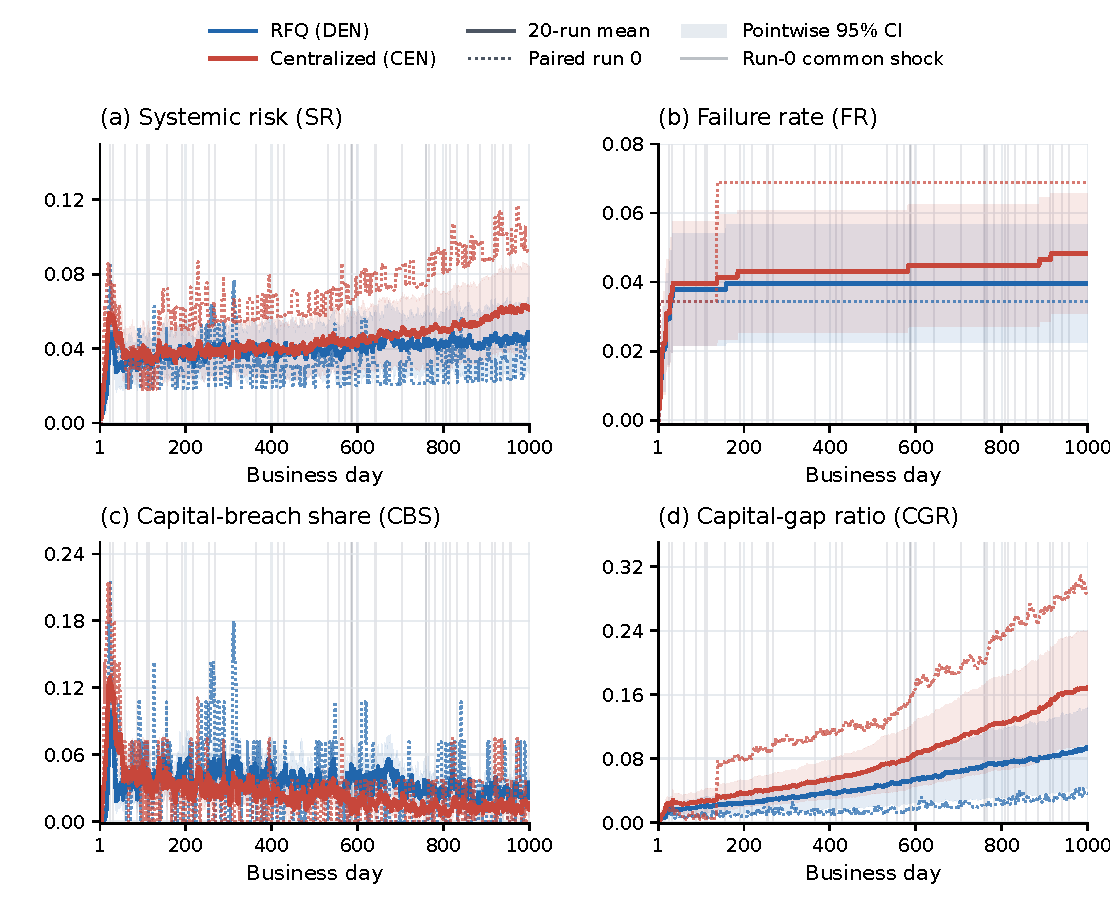
\includegraphics[width=\textwidth]{figures/compare_baseline_rollover_on_support_on.pdf}
\caption{Baseline ON/ON trajectories under decentralized RFQ and centralized matching. Solid lines are means of all 20 paired replications, which contribute at every date through day 1000; dotted lines show paired run 0; shaded regions are pointwise normal-approximation 95\% intervals.
CBS uses active banks and the recovery rule in Chapter~3; CGR uses gap
divided by required capital. Pale vertical lines mark common-shock dates
in paired run 0.}
\label{fig:baseline-on-on}
\end{figure}

The average full-horizon systemic-risk level is 0.0396 under RFQ and
0.0447 under centralized matching. The mean paired difference is
\(-0.00513\), and its 95\% paired interval is
\([-0.01276,0.00249]\). Integrated risk gives the equivalent result in
business-day units: the mean RFQ-minus-Centralized AUC difference is
\(-5.12\), with interval \([-12.74,2.49]\). At day 1000, mean SR is
0.0449 under RFQ and 0.0622 under centralized matching; the paired
difference is \(-0.01727\), with interval \([-0.03233,-0.00222]\).
Thus the full-horizon mean is directionally lower but not statistically
separated, whereas the day-1000 paired difference excludes zero.

\begin{table}[htbp]
\centering
\caption{Paired ON/ON systemic-risk comparison over 1000 business days}
\label{tab:paired-baseline-risk}
\scriptsize
\begin{tabularx}{\textwidth}{@{}>{\raggedright\arraybackslash}Xrr>{\raggedleft\arraybackslash}p{0.34\textwidth}@{}}
\toprule
\textbf{Measure} & \textbf{RFQ} & \textbf{Centralized} & \textbf{RFQ--Centralized (95\% CI)}\\
\midrule
Mean SR over time & 0.0396 & 0.0447 & $-0.00513$ $[-0.01276,\ 0.00249]$\\
AUC of SR & 39.55 & 44.68 & $-5.12$ $[-12.74,\ 2.49]$\\
SR at day 1000 & 0.0449 & 0.0622 & $-0.01727$ $[-0.03233,\ -0.00222]$\\
Median SR at day 1000 & 0.0313 & 0.0481 & $-0.00099$\\
Mean CGR over time & 0.0479 & 0.0782 & $-0.03028$ $[-0.05229,\ -0.00827]$\\
CGR at day 1000 & 0.0932 & 0.1688 & $-0.07555$ $[-0.12626,\ -0.02484]$\\
Median CGR at day 1000 & 0.0547 & 0.0924 & $-0.00663$\\
\bottomrule
\end{tabularx}
\begin{minipage}{0.96\textwidth}
\footnotesize
\textit{Note:} \(N=20\) paired seeds. Confidence intervals are paired
normal-approximation intervals. The two mechanism columns report
medians of their day-1000 values. In each median row, the difference column
reports \(\operatorname{median}_m(\mathrm{RFQ}_m-\mathrm{CEN}_m)\),
which need not equal the difference between the two marginal medians.
\end{minipage}
\end{table}

Figure~\ref{fig:paired-sr-on-on} shows the paired difference day by day.
It is negative over most of the horizon and becomes more negative in the
later portion, but its pointwise interval frequently crosses zero. The
correct conclusion is therefore directional: RFQ has lower estimated
systemic risk in this sample, with the clearest statistically separated
effect appearing in the final capital-gap ratio rather than in the
composite index at every date.

\begin{figure}[htbp]
\centering
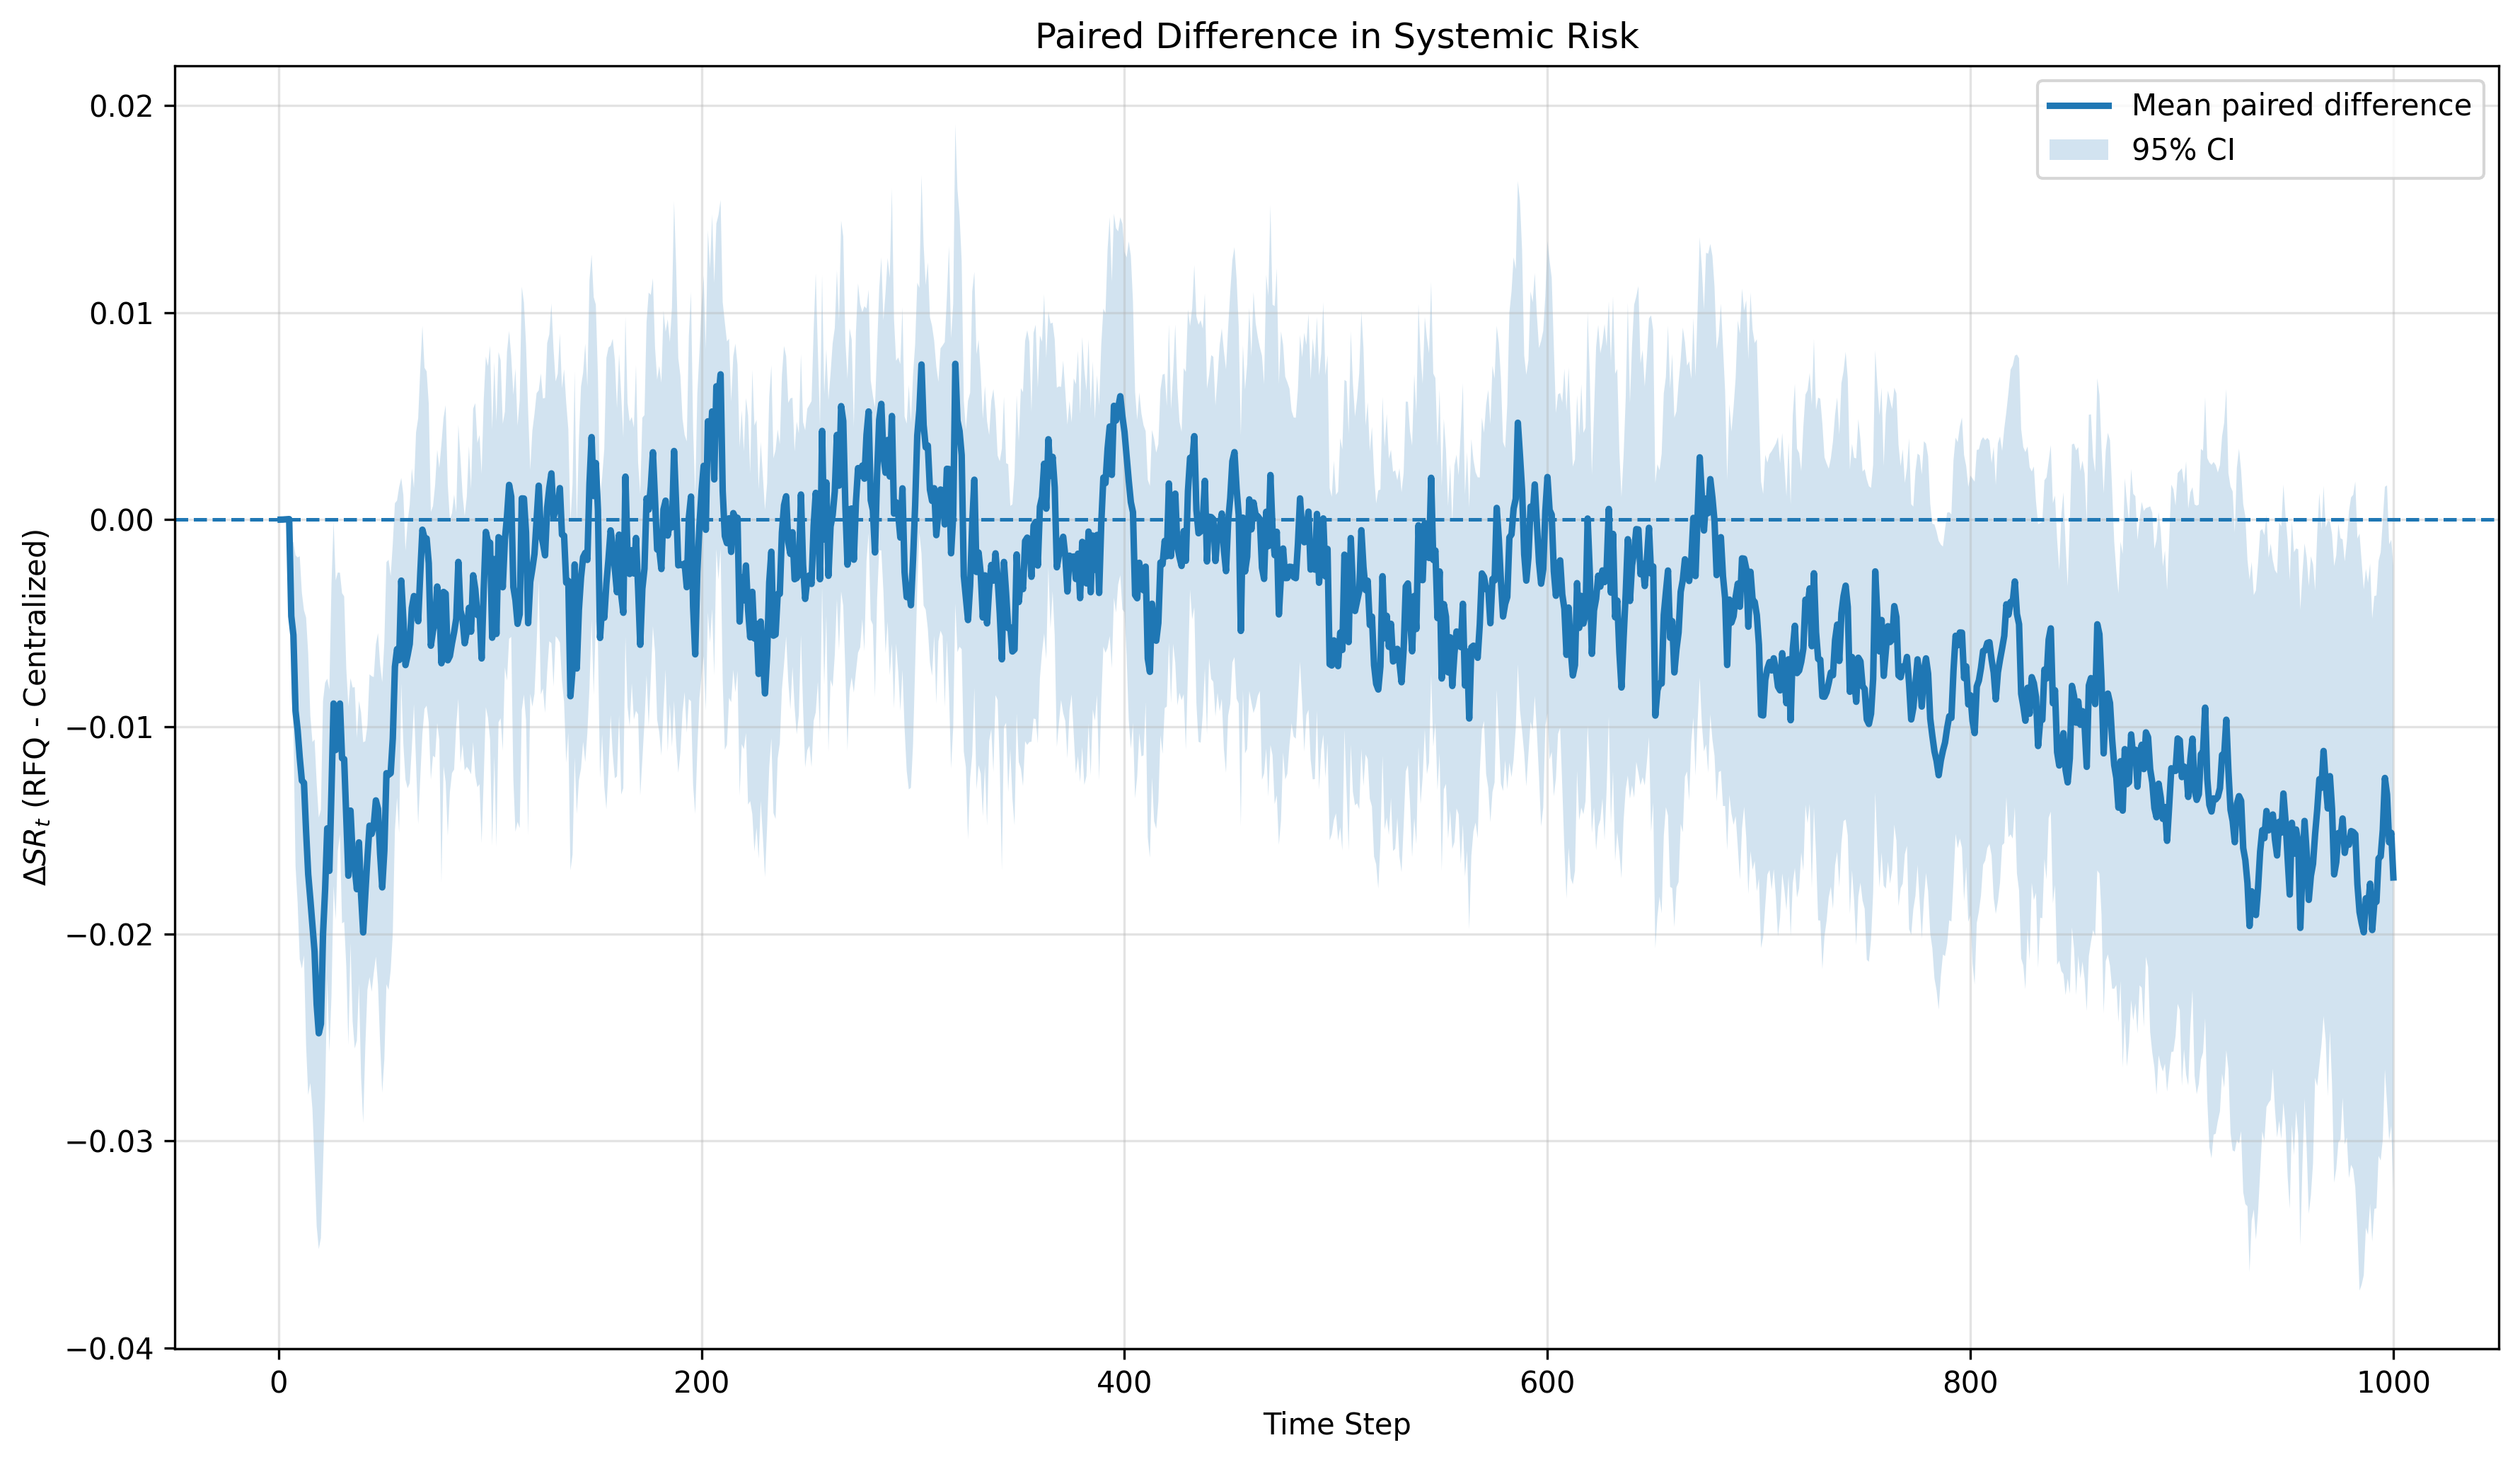
\includegraphics[width=0.92\textwidth]{figures/paired_sr_difference_rollover_on_support_on.png}
\caption{Paired RFQ-minus-Centralized difference in systemic risk under ON/ON. Negative values favor RFQ. All 20 pairs contribute at every date through day 1000; the shaded region is the pointwise 95\% interval.}
\label{fig:paired-sr-on-on}
\end{figure}

Table~\ref{tab:first-passage} reports first-passage and hit-rate outcomes
for the ON/ON sample. The failure-rate thresholds \(\mathrm{FR}_t\geq 0.5\)
and \(\mathrm{FR}_t\geq 0.9\) are never reached, and no replication hits
\(\mathrm{SR}_t\geq 0.20\). Conditional arrival times at those thresholds
are therefore unidentified: the hit rate is the identified object, and it
equals zero. Lower composite-risk thresholds do produce hits.
\(\mathrm{SR}_t\geq 0.05\) is reached in 15 of 20 RFQ runs and 17 of 20
centralized runs. Among the 15 paired replications in which both
mechanisms hit, RFQ arrives 16.6 days later on average, with paired-bootstrap
interval \([4.5,31.8]\). At \(\mathrm{SR}_t\geq 0.08\) the hit rate is 0.50
for both mechanisms; the dual-hit delay is \(+118.8\) days
\([9.0,266.0]\) on nine pairs. At \(\mathrm{SR}_t\geq 0.10\) the dual-hit
delay is \(+128.0\) days \([59.8,194.7]\) on six pairs. Positive paired
delays mean that RFQ reaches the threshold later.

\begin{table}[htbp]
\centering
\caption{ON/ON first-passage times, hit rates, and paired delays}
\label{tab:first-passage}
\small
\setlength{\tabcolsep}{4pt}
\begin{tabularx}{\textwidth}{@{}lcccc>{\centering\arraybackslash}X@{}}
\toprule
\textbf{Threshold} & \textbf{RFQ hit} & \textbf{CEN hit} & \shortstack{\textbf{RFQ mean}\\\(\tau\)} & \shortstack{\textbf{CEN mean}\\\(\tau\)} & \textbf{Paired delay}\\
\midrule
$\mathrm{FR}_t\geq 0.50$ & 0.00 & 0.00 & -- & -- & --\\
$\mathrm{FR}_t\geq 0.90$ & 0.00 & 0.00 & -- & -- & --\\
Collapse (recorded stop) & 0.00 & 0.00 & -- & -- & --\\
$\mathrm{SR}_t\geq 0.05$ & 0.75 & 0.85 & 43.8 & 26.6 & $+16.6$ $[4.5,\ 31.8]$\\
$\mathrm{SR}_t\geq 0.08$ & 0.50 & 0.50 & 189.8 & 124.8 & $+118.8$ $[9.0,\ 266.0]$\\
$\mathrm{SR}_t\geq 0.10$ & 0.30 & 0.45 & 240.7 & 270.2 & $+128.0$ $[59.8,\ 194.7]$\\
$\mathrm{SR}_t\geq 0.20$ & 0.00 & 0.00 & -- & -- & --\\
\bottomrule
\end{tabularx}
\begin{minipage}{0.96\textwidth}
\footnotesize
\textit{Note:} \(N=20\). Hit-conditional means use all replications that
reach the threshold. Paired delays are RFQ minus Centralized first-passage
times on dual-hit pairs only (\(n=15\), \(9\), and \(6\)). Positive values
mean RFQ arrives later. Intervals are paired-bootstrap percentile 95\%
intervals. Conditional medians at \(\mathrm{SR}\ge 0.05/0.08/0.10\) are
22, 36.5, and 158.5 under RFQ and 21, 21.5, and 34 under centralized
matching. Dashes indicate that the arrival time is unidentified.
\end{minipage}
\end{table}

\section{Network Formation and Funding Outcomes}

The aggregate risk difference is modest, but the two mechanisms produce
materially different interbank networks. Figures~\ref{fig:network-den20}--
\ref{fig:network-cen200} show enlarged representative snapshots at steps
20 and 200, while Table~\ref{tab:network-results} summarizes full-horizon,
replication-level statistics. Each snapshot is presented separately so
that bank labels, node-level risk values, and bilateral links remain
legible in print.

\begin{figure}[p]
\centering
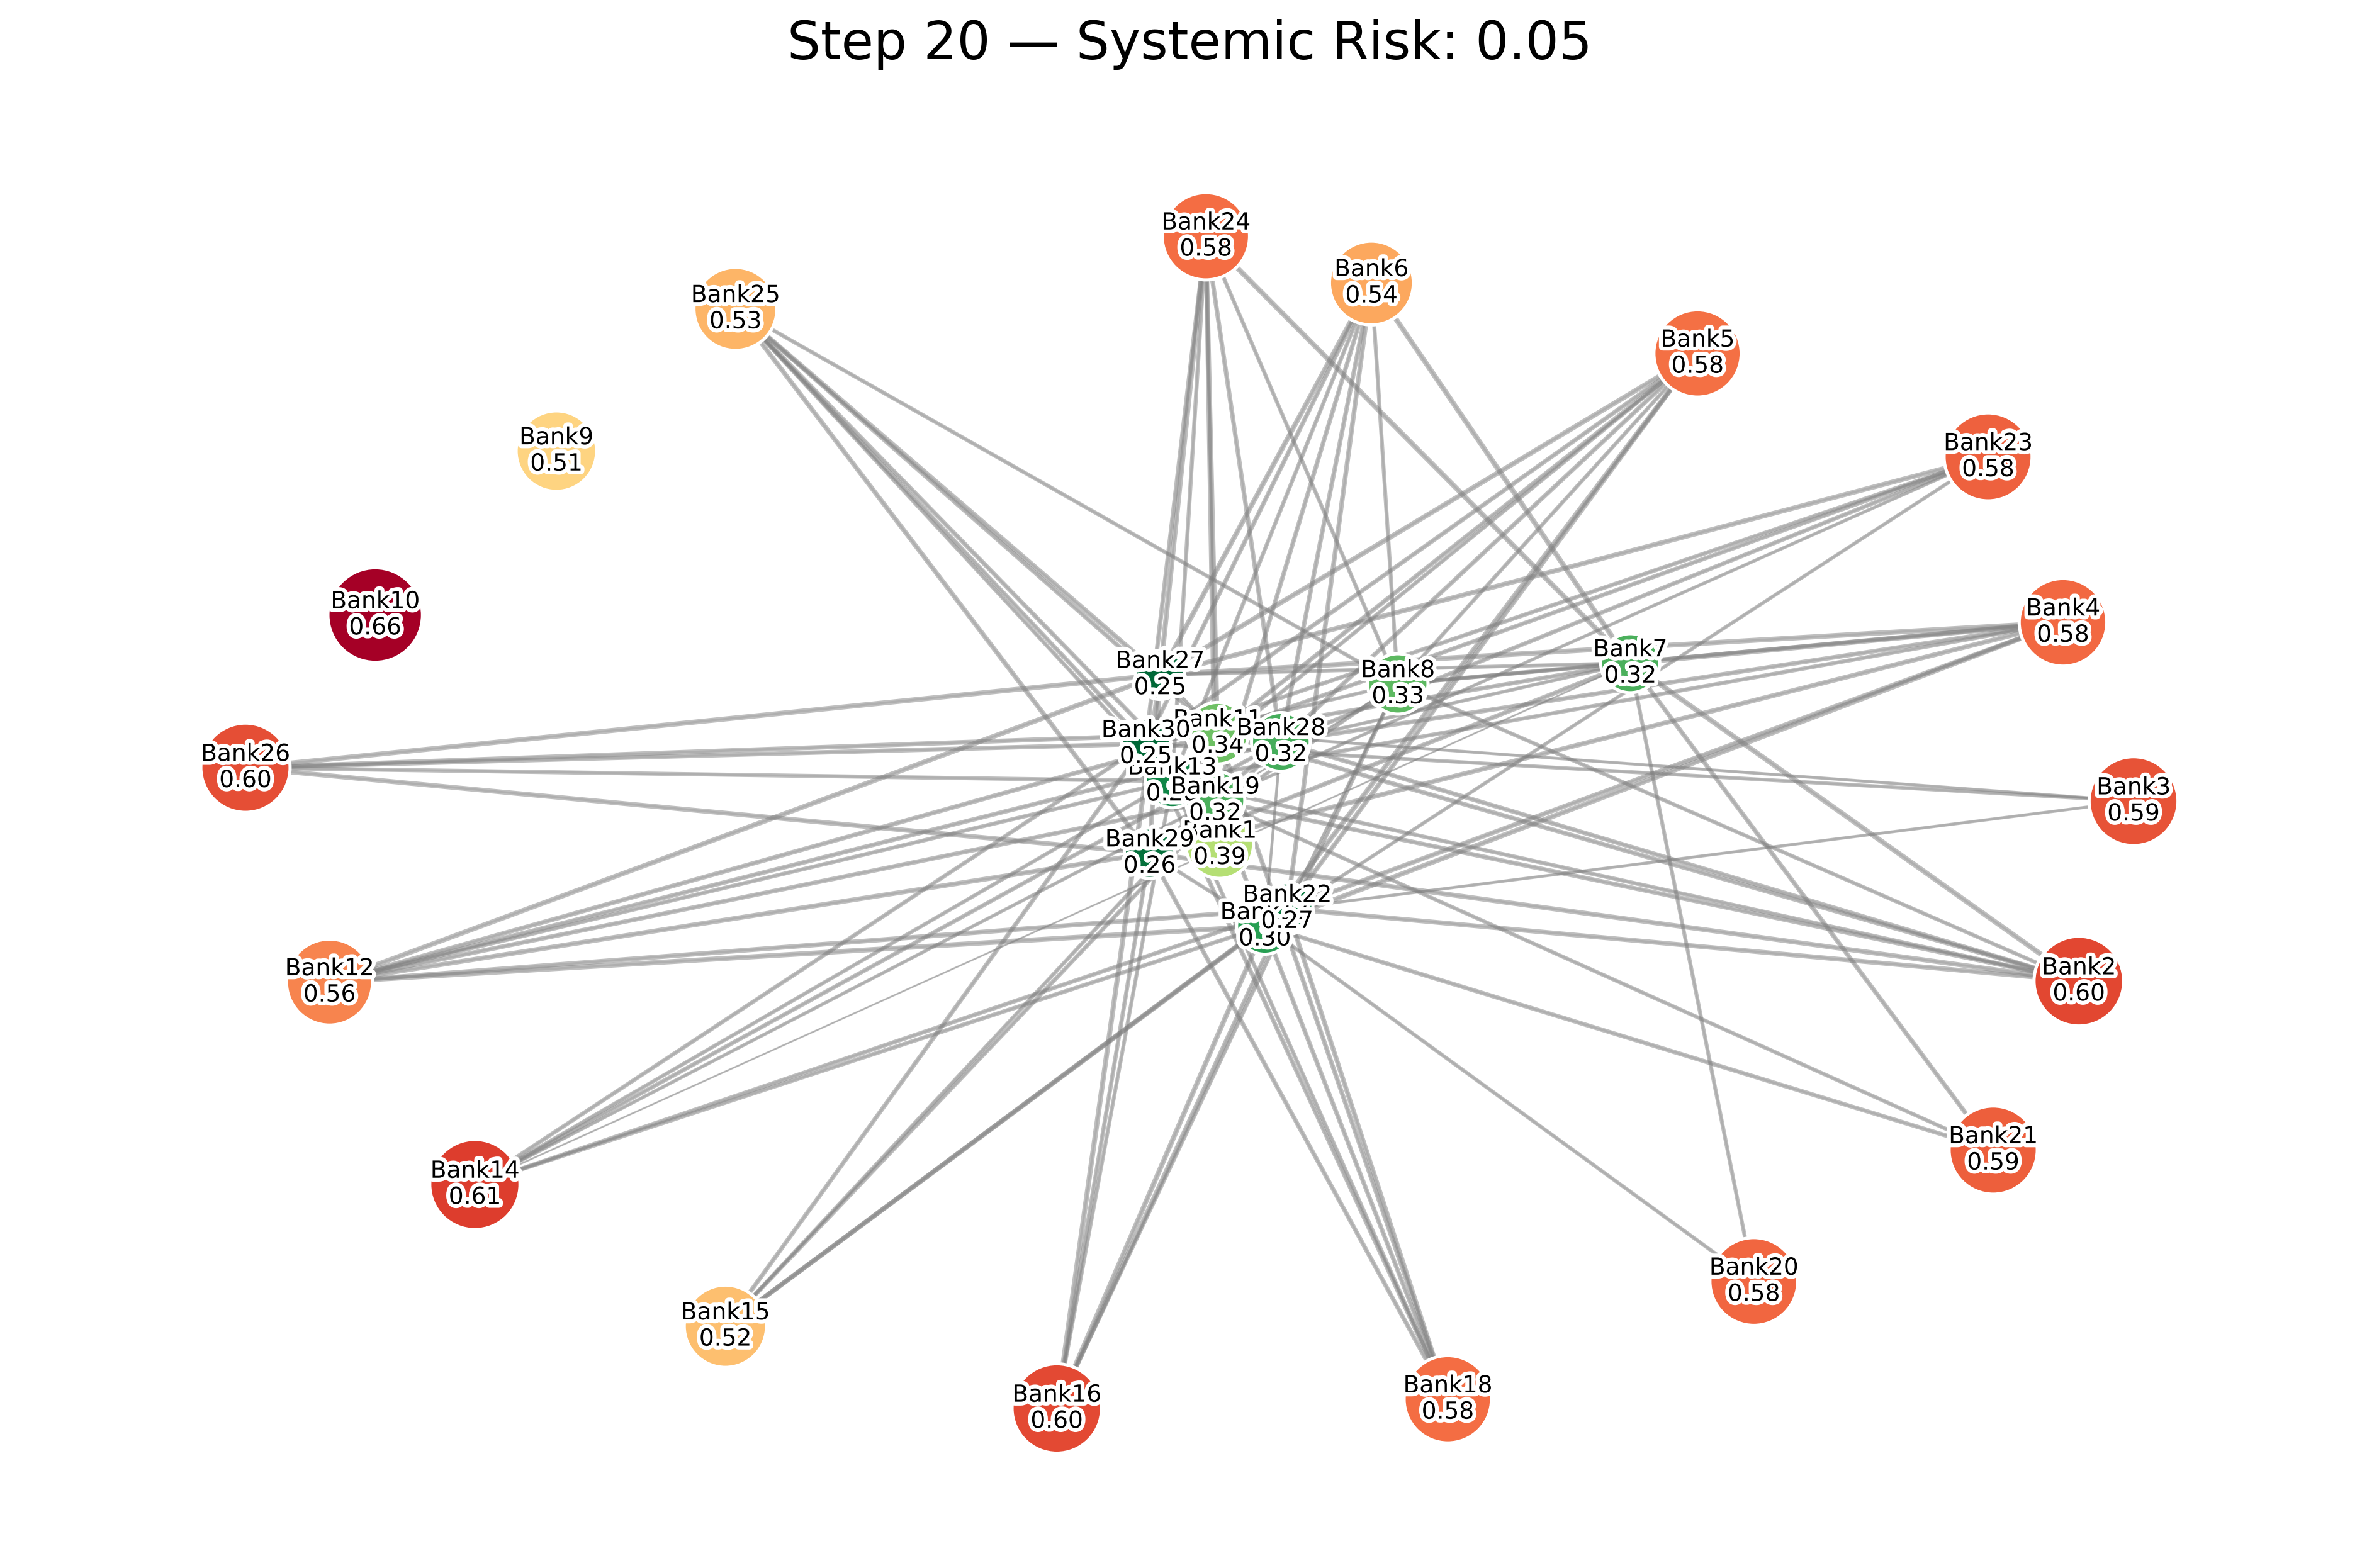
\includegraphics[width=0.96\textwidth]{figures/network_decentralized_step20.png}
\caption{Outstanding interbank exposures under decentralized RFQ at step 20 in the ON/ON scenario (SR = 0.05).}
\label{fig:network-den20}
\end{figure}

\begin{figure}[p]
\centering
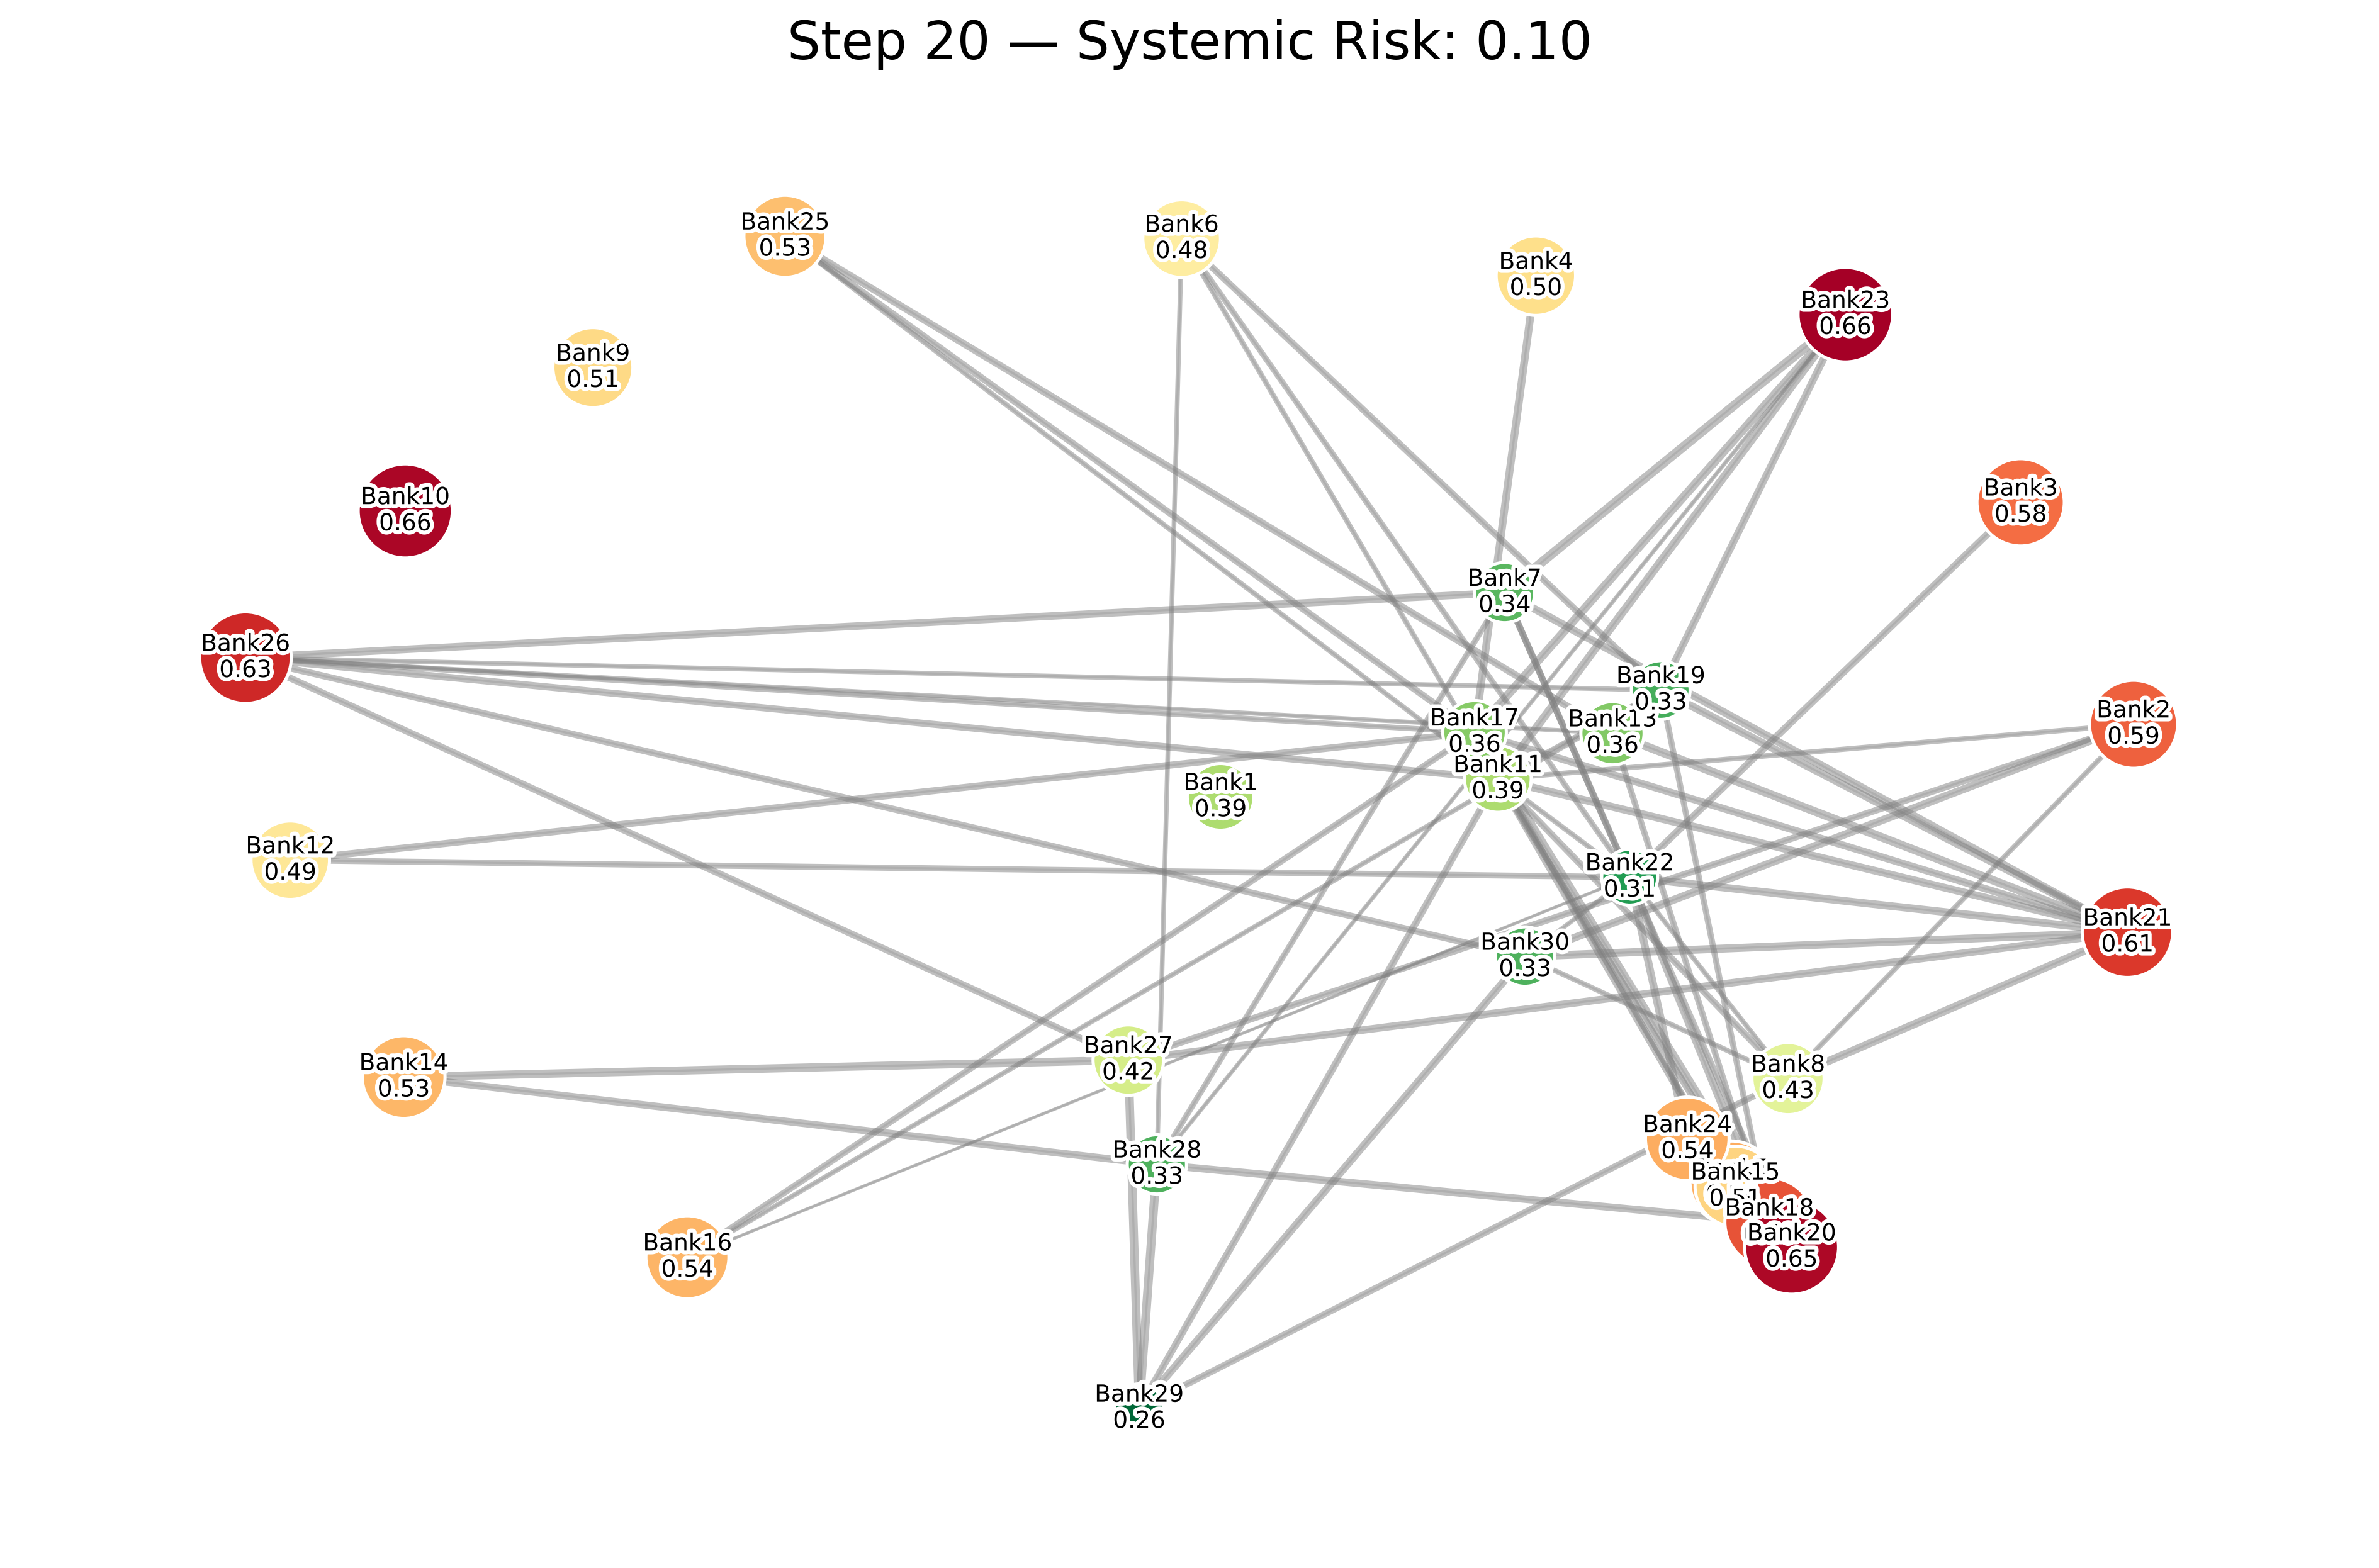
\includegraphics[width=0.96\textwidth]{figures/network_centralized_step20.png}
\caption{Outstanding interbank exposures under centralized matching at step 20 in the ON/ON scenario (SR = 0.10).}
\label{fig:network-cen20}
\end{figure}

\begin{figure}[p]
\centering
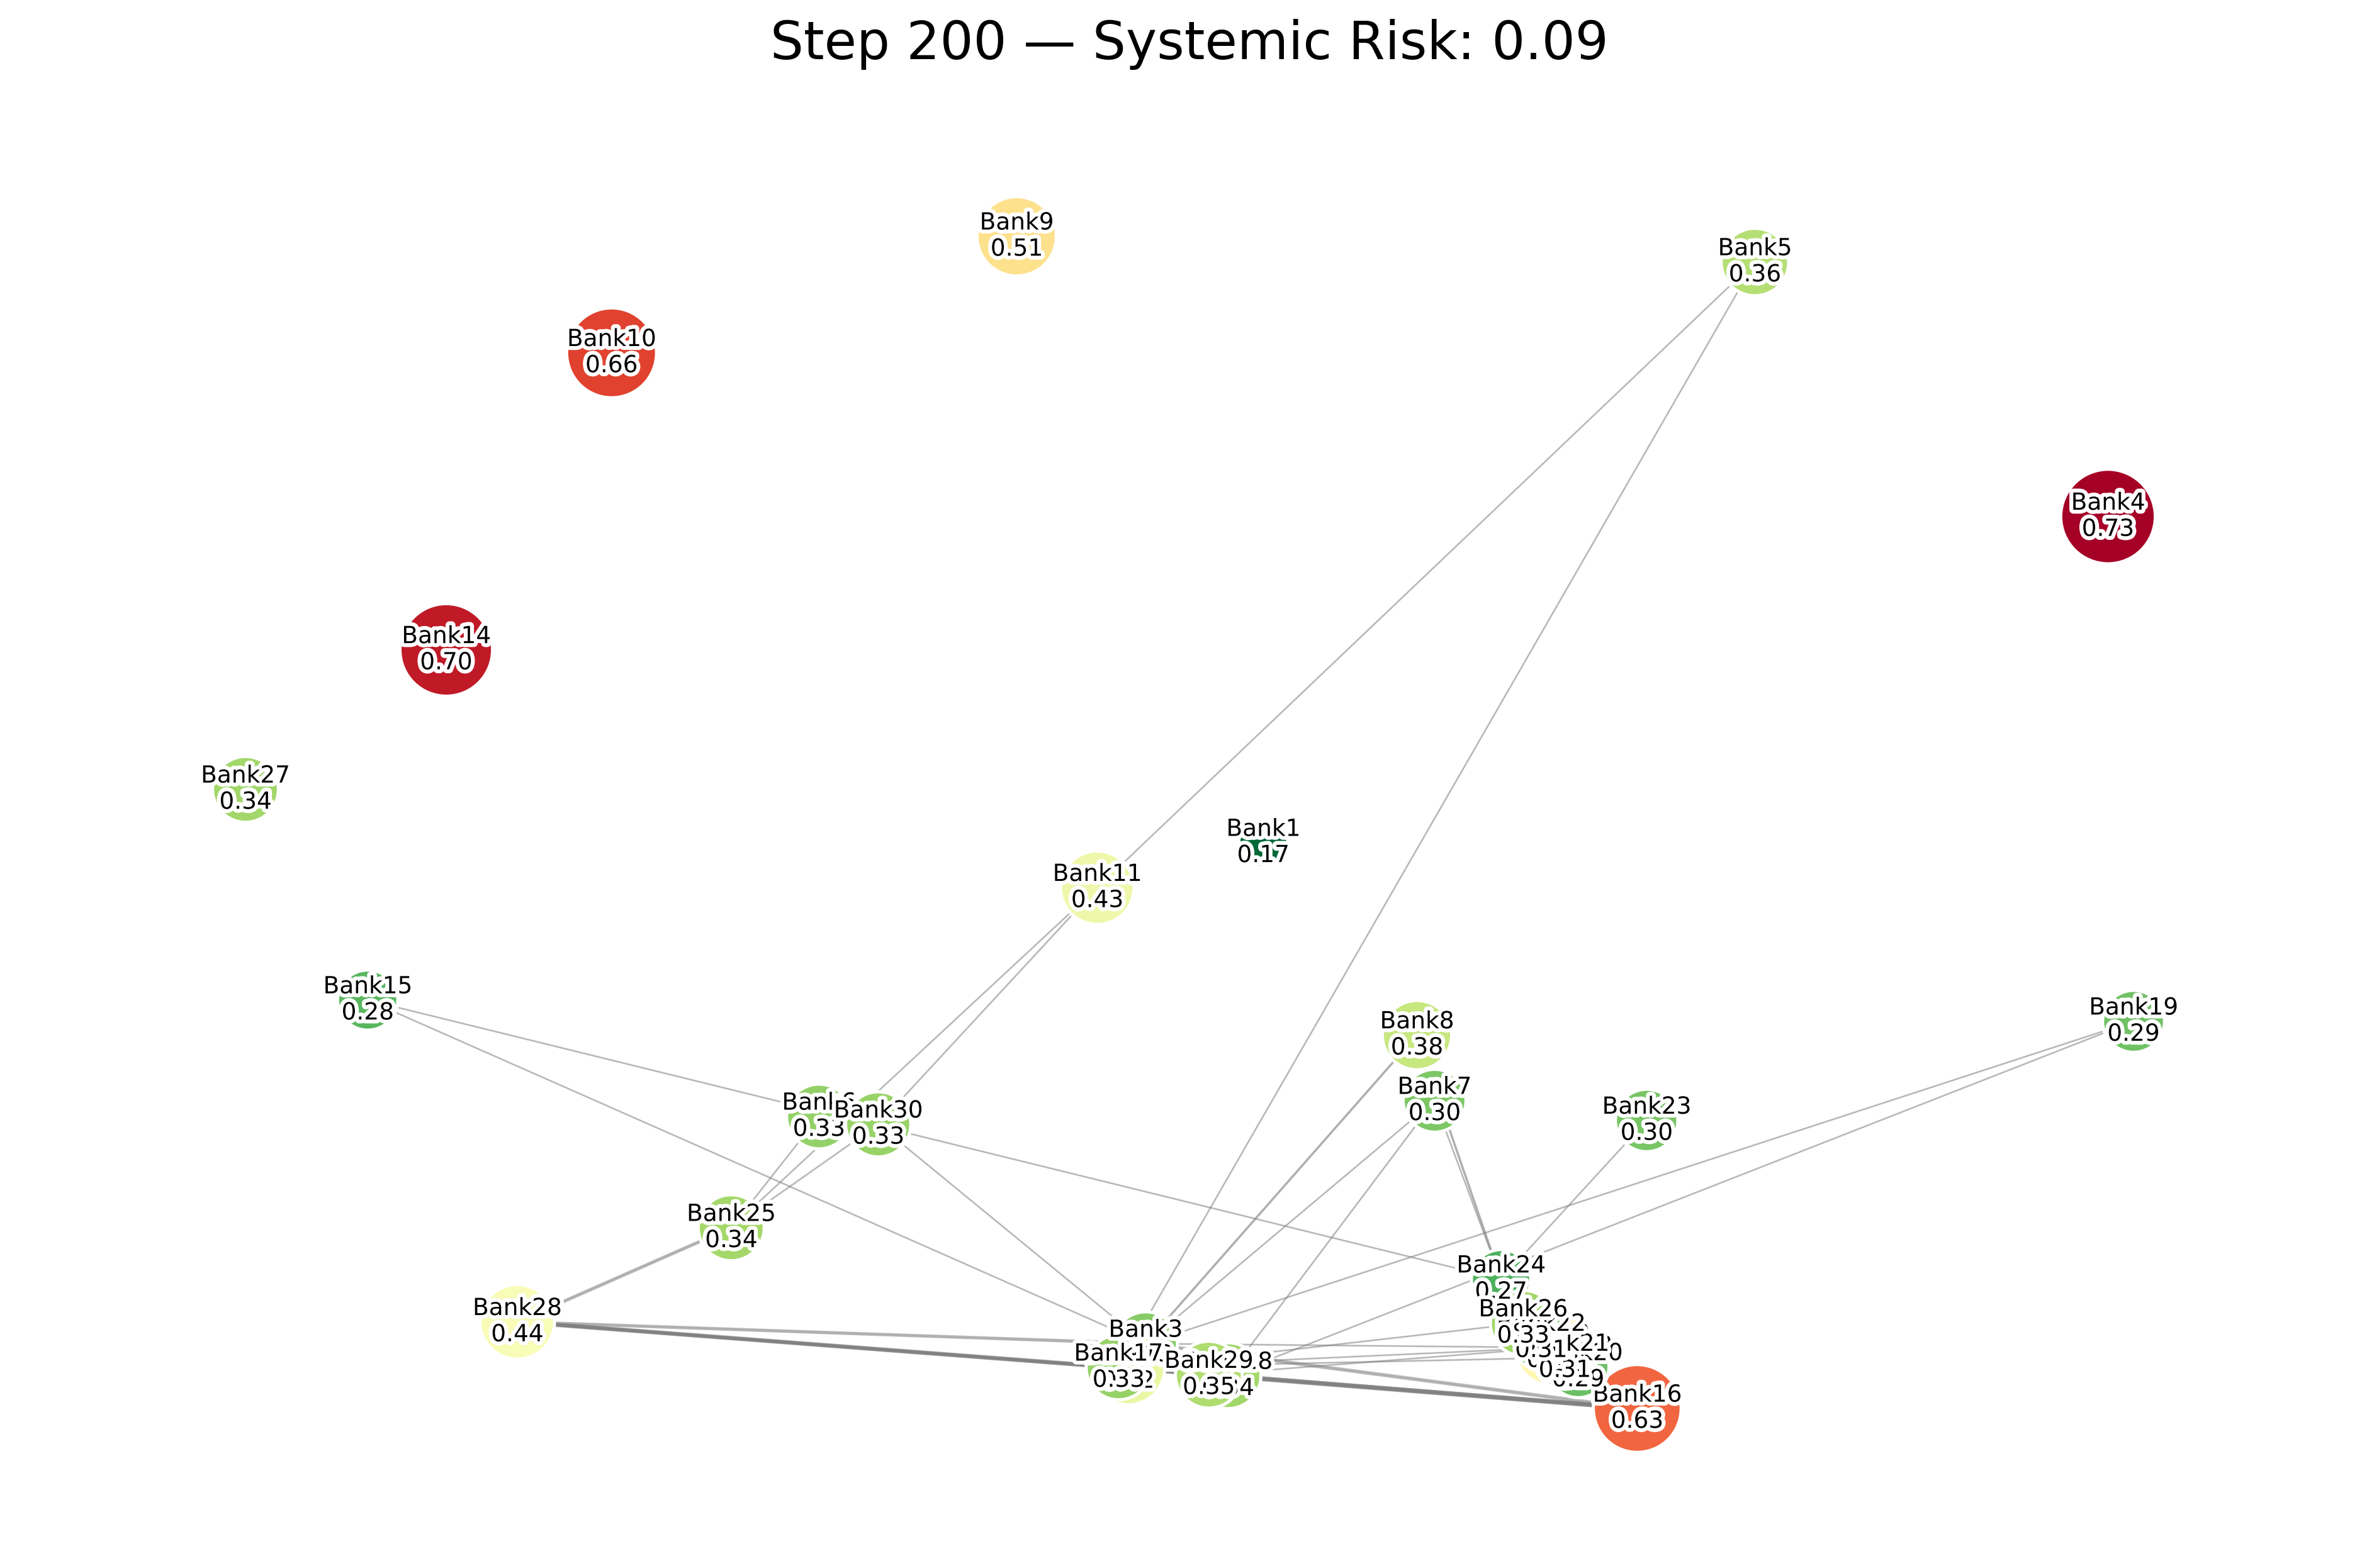
\includegraphics[width=0.96\textwidth]{figures/network_decentralized_step200.png}
\caption{Outstanding interbank exposures under decentralized RFQ at step 200 in the ON/ON scenario (SR = 0.09).}
\label{fig:network-den200}
\end{figure}

\begin{figure}[p]
\centering
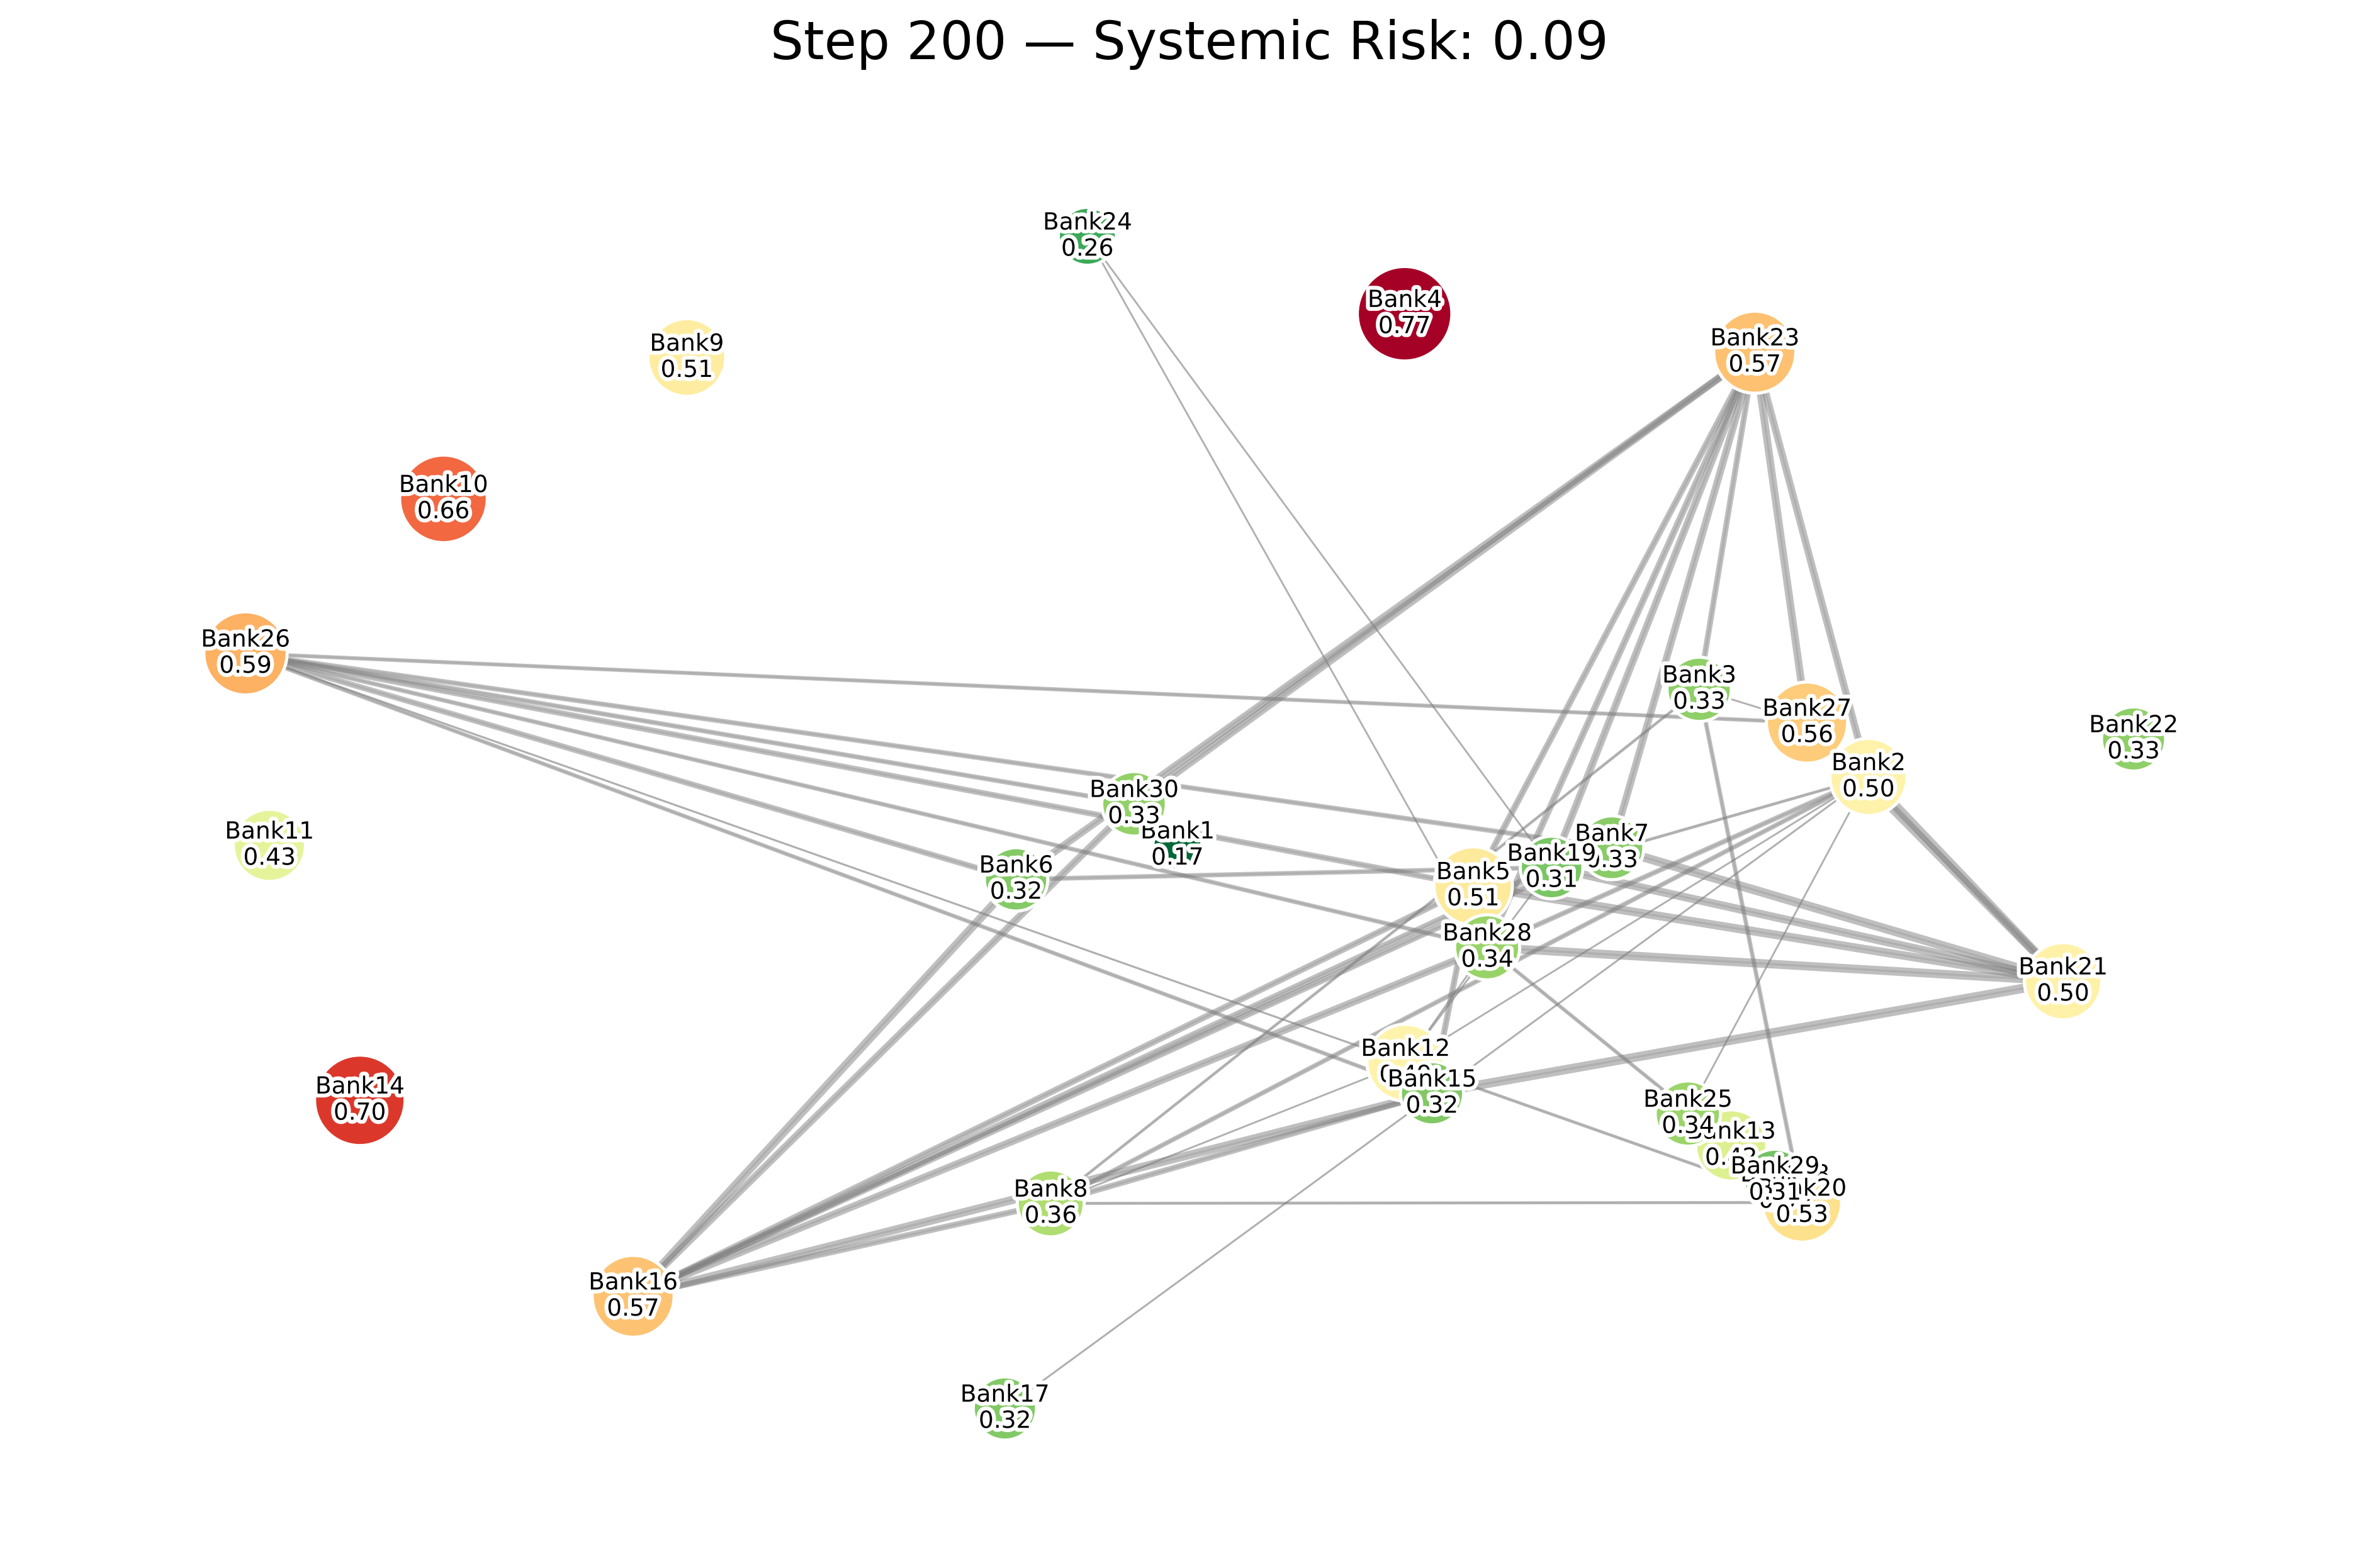
\includegraphics[width=0.96\textwidth]{figures/network_centralized_step200.png}
\caption{Outstanding interbank exposures under centralized matching at step 200 in the ON/ON scenario (SR = 0.09).}
\label{fig:network-cen200}
\end{figure}

\begin{table}[htbp]
\centering
\caption{Paired ON/ON network and funding statistics}
\label{tab:network-results}
\small
\begin{tabular}{@{}lrrr@{}}
\toprule
\textbf{Measure} & \textbf{RFQ} & \textbf{Centralized} & \textbf{RFQ--Centralized (95\% CI)}\\
\midrule
Active directed links & 58.95 & 37.77 & $21.19$ $[14.13,\ 28.24]$\\
Network density & 0.0726 & 0.0465 & $0.0261$ $[0.0174,\ 0.0348]$\\
Mean degree & 4.066 & 2.605 & $1.461$ $[0.975,\ 1.948]$\\
Degree dispersion & 2.943 & 2.562 & $0.381$ $[0.150,\ 0.613]$\\
Mean weighted degree & 86.70 & 90.90 & $-4.20$ $[-18.78,\ 10.38]$\\
Largest bilateral exposure & 115.89 & 1,118.80 & $-1{,}002.91$ $[-1{,}167.96,\ -837.87]$\\
Exposure HHI & 0.050 & 0.094 & $-0.0435$ $[-0.0572,\ -0.0298]$\\
Largest component size & 24.03 & 17.08 & $6.95$ $[4.79,\ 9.10]$\\
Funding satisfaction & 0.530 & 0.597 & $-0.067$ $[-0.111,\ -0.024]$\\
Cumulative volume & 325,406 & 314,721 & $10{,}685$ $[-41{,}740,\ 63{,}110]$\\
\bottomrule
\end{tabular}
\begin{minipage}{0.96\textwidth}
\footnotesize
\textit{Note:} Entries are means across 20 paired replications. Network
measures are averaged over the observed days within each replication;
funding satisfaction is the event-conditional daily ratio; volume is the
calendar-day cumulative total. Intervals are paired normal-approximation
95\% intervals for RFQ-minus-Centralized differences.
\end{minipage}
\end{table}

RFQ therefore forms more links and a larger connected component while
producing substantially lower bilateral-exposure concentration. Its
funding-satisfaction ratio is lower, but cumulative volume is similar:
the paired volume interval includes zero. The market-wide centralized
rule directs much larger amounts to individual bilateral exposures,
whereas RFQ spreads transactions across a broader set of counterparties.
This diversification is the main structural mechanism consistent with
RFQ's lower capital-gap point estimate; it is not evidence that RFQ
dominates funding completion.

\section{Response to Common Shocks}

The common-shock event study pools approximately 698 shock events across
the 20 paired paths. Figure~\ref{fig:shock-study} aligns each event at
\(\tau=0\) and reports two pre-event and five post-event business days.

\begin{figure}[htbp]
\centering
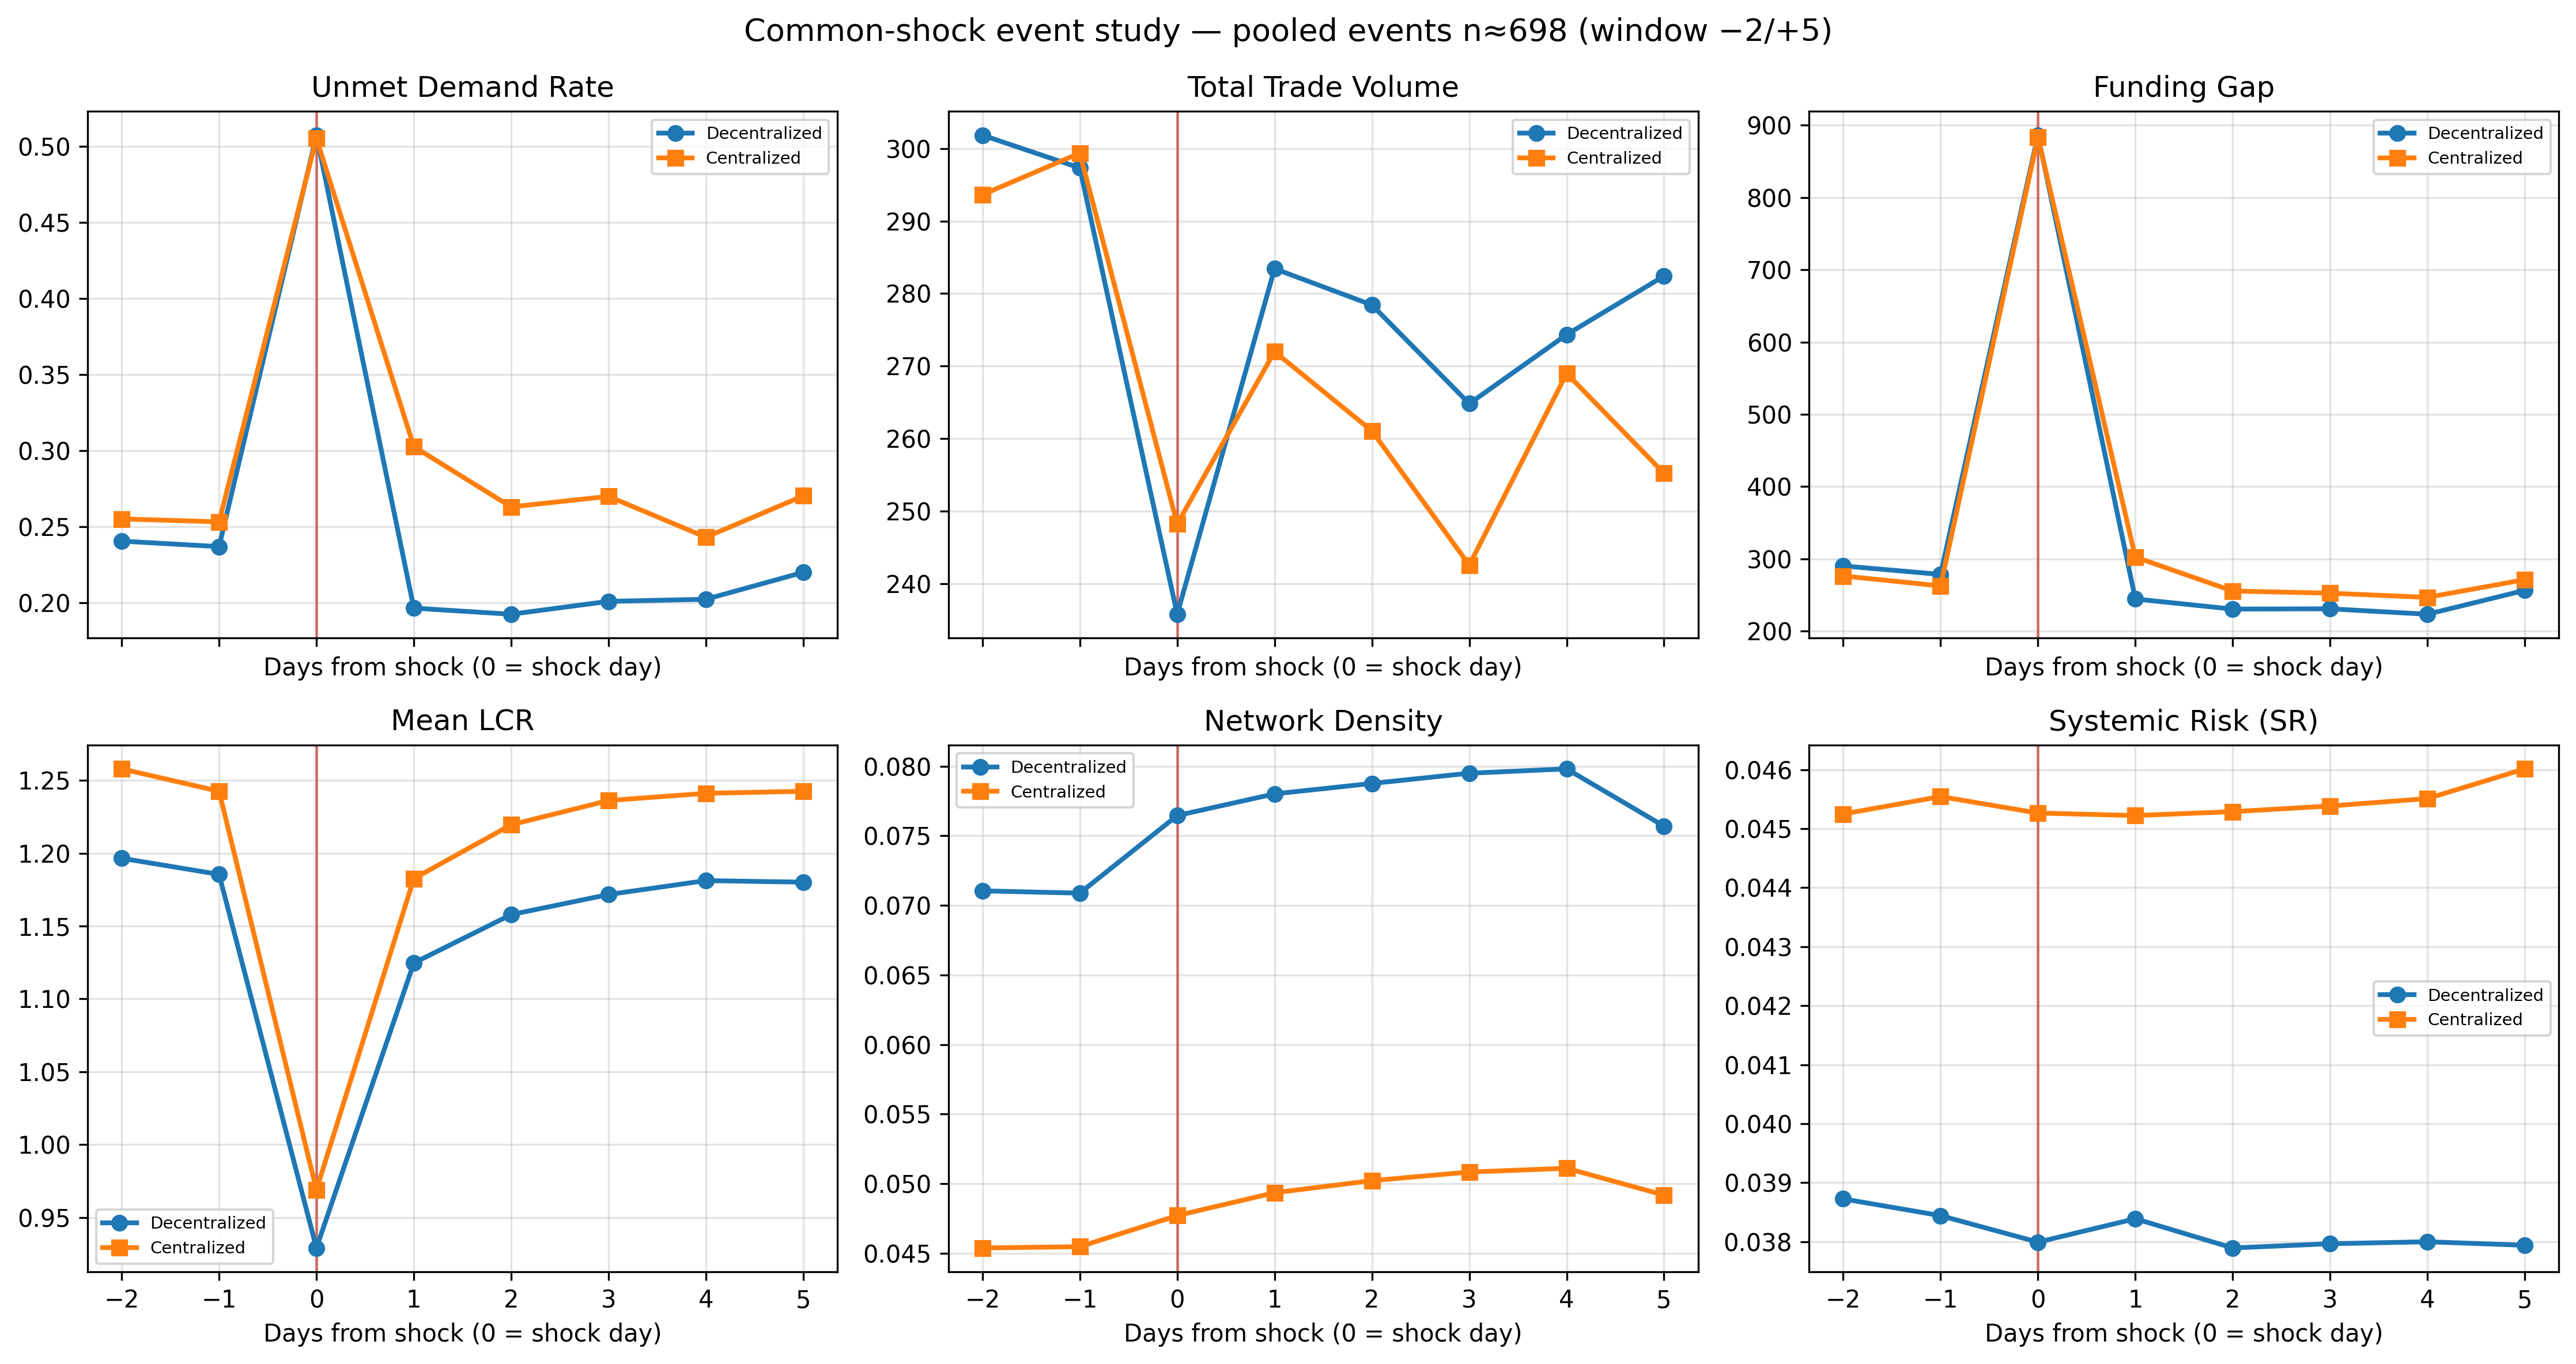
\includegraphics[width=\textwidth]{figures/compare_shock_event_study_rollover_on_support_on.png}
\caption{Pooled response to common liquidity-and-credit shocks in the ON/ON scenario. The event date is \(\tau=0\).}
\label{fig:shock-study}
\end{figure}

On the shock date, the unmet-demand rate rises to approximately 0.50 and
the funding gap to approximately 884--886 under both mechanisms. Mean LCR
falls sharply, to 0.929 in RFQ and 0.969 in centralized matching. The
mechanism difference appears in recovery. At \(\tau=1\), unmet demand is
0.196 under RFQ and 0.303 under centralized matching, while the funding
gap is 244 versus 302. RFQ network density rises from 0.071 before the
shock to 0.076 on the event date and remains near 0.078--0.079 over the
next four days; centralized density rises more modestly from 0.045 to
0.048--0.051. Mean SR remains around 0.038 under RFQ and 0.045--0.046
under centralized matching. These results suggest that RFQ's broader but
less concentrated set of local links supports post-shock reallocation,
even though both designs experience the same initial common funding
pressure.

\section{Rollover and Policy-Support Interaction}

The four configurations combine rollover ON/OFF with policy support
ON/OFF. Figures~\ref{fig:four-den} and \ref{fig:four-cen} show the
mechanism-specific comparisons. Because rollover selects the contract
schedule at origination, ON means 5--20-period installments and OFF means
next-day single payment. Support ON adds next-day liquidity assistance
and post-project solvency support subject to finite budgets.

\begin{figure}[htbp]
\centering
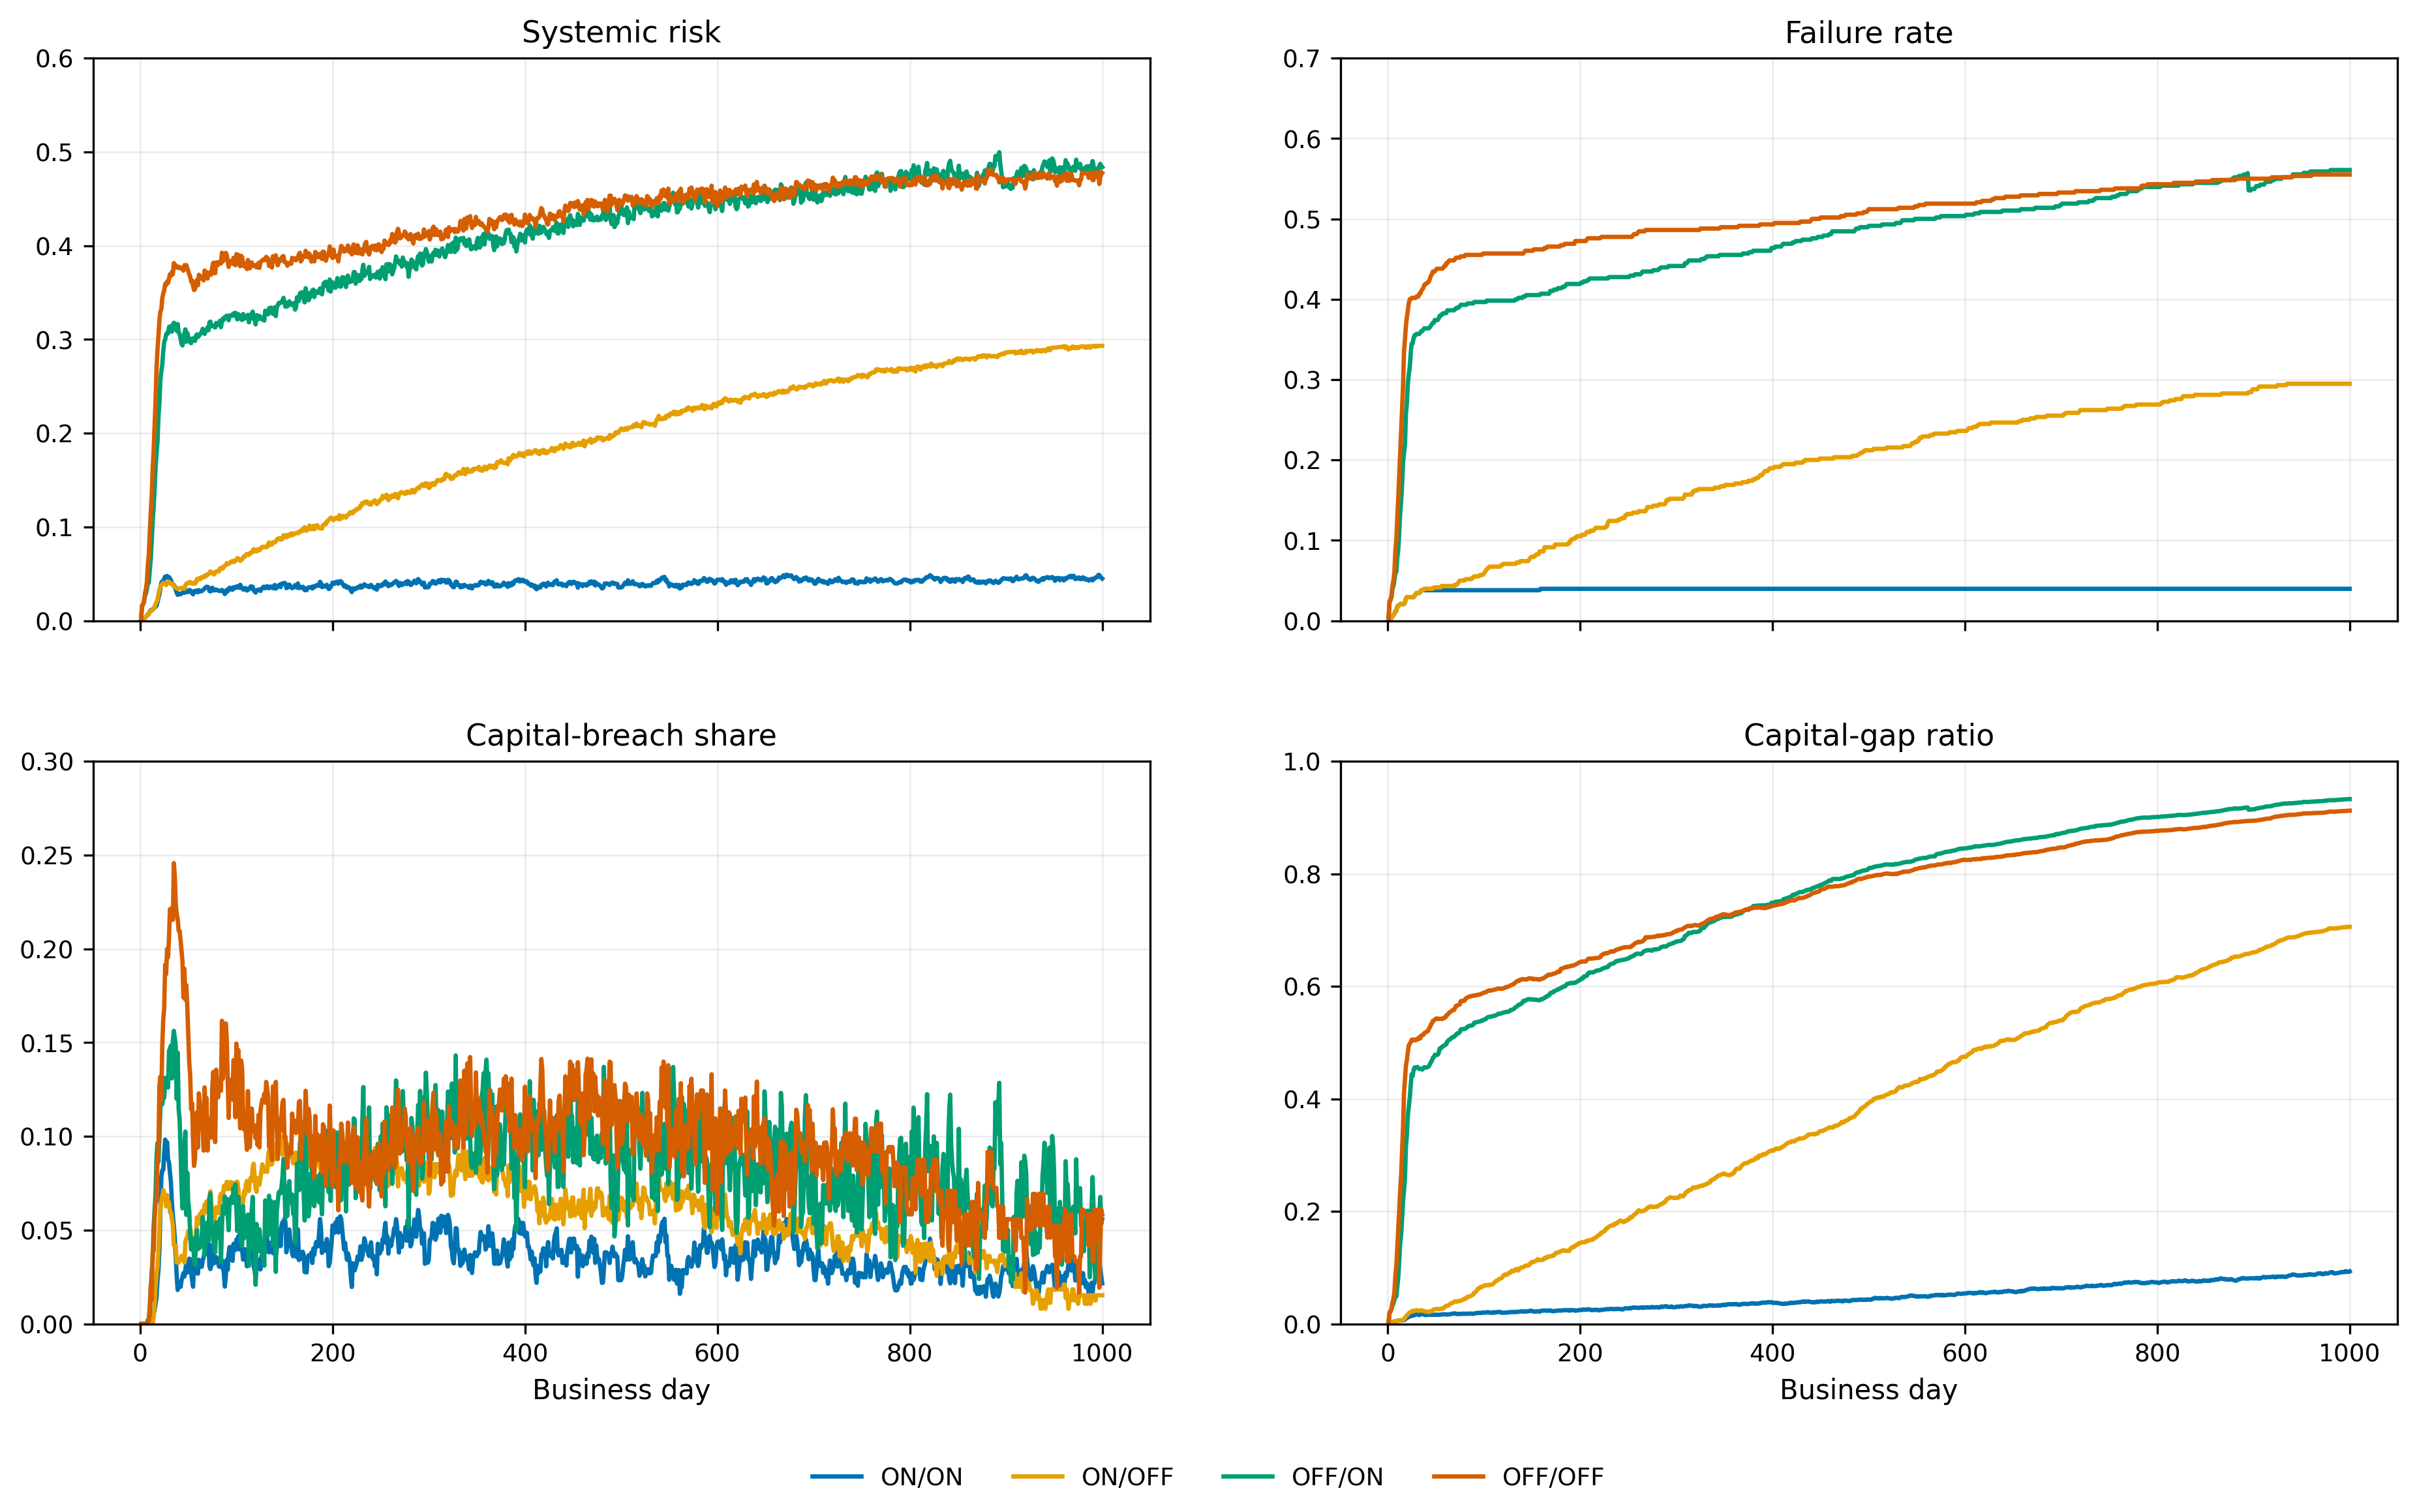
\includegraphics[width=0.96\textwidth]{figures/compare_four_baselines_decentralized.png}
\caption{Four rollover/support configurations under decentralized RFQ.}
\label{fig:four-den}
\end{figure}

\begin{figure}[htbp]
\centering
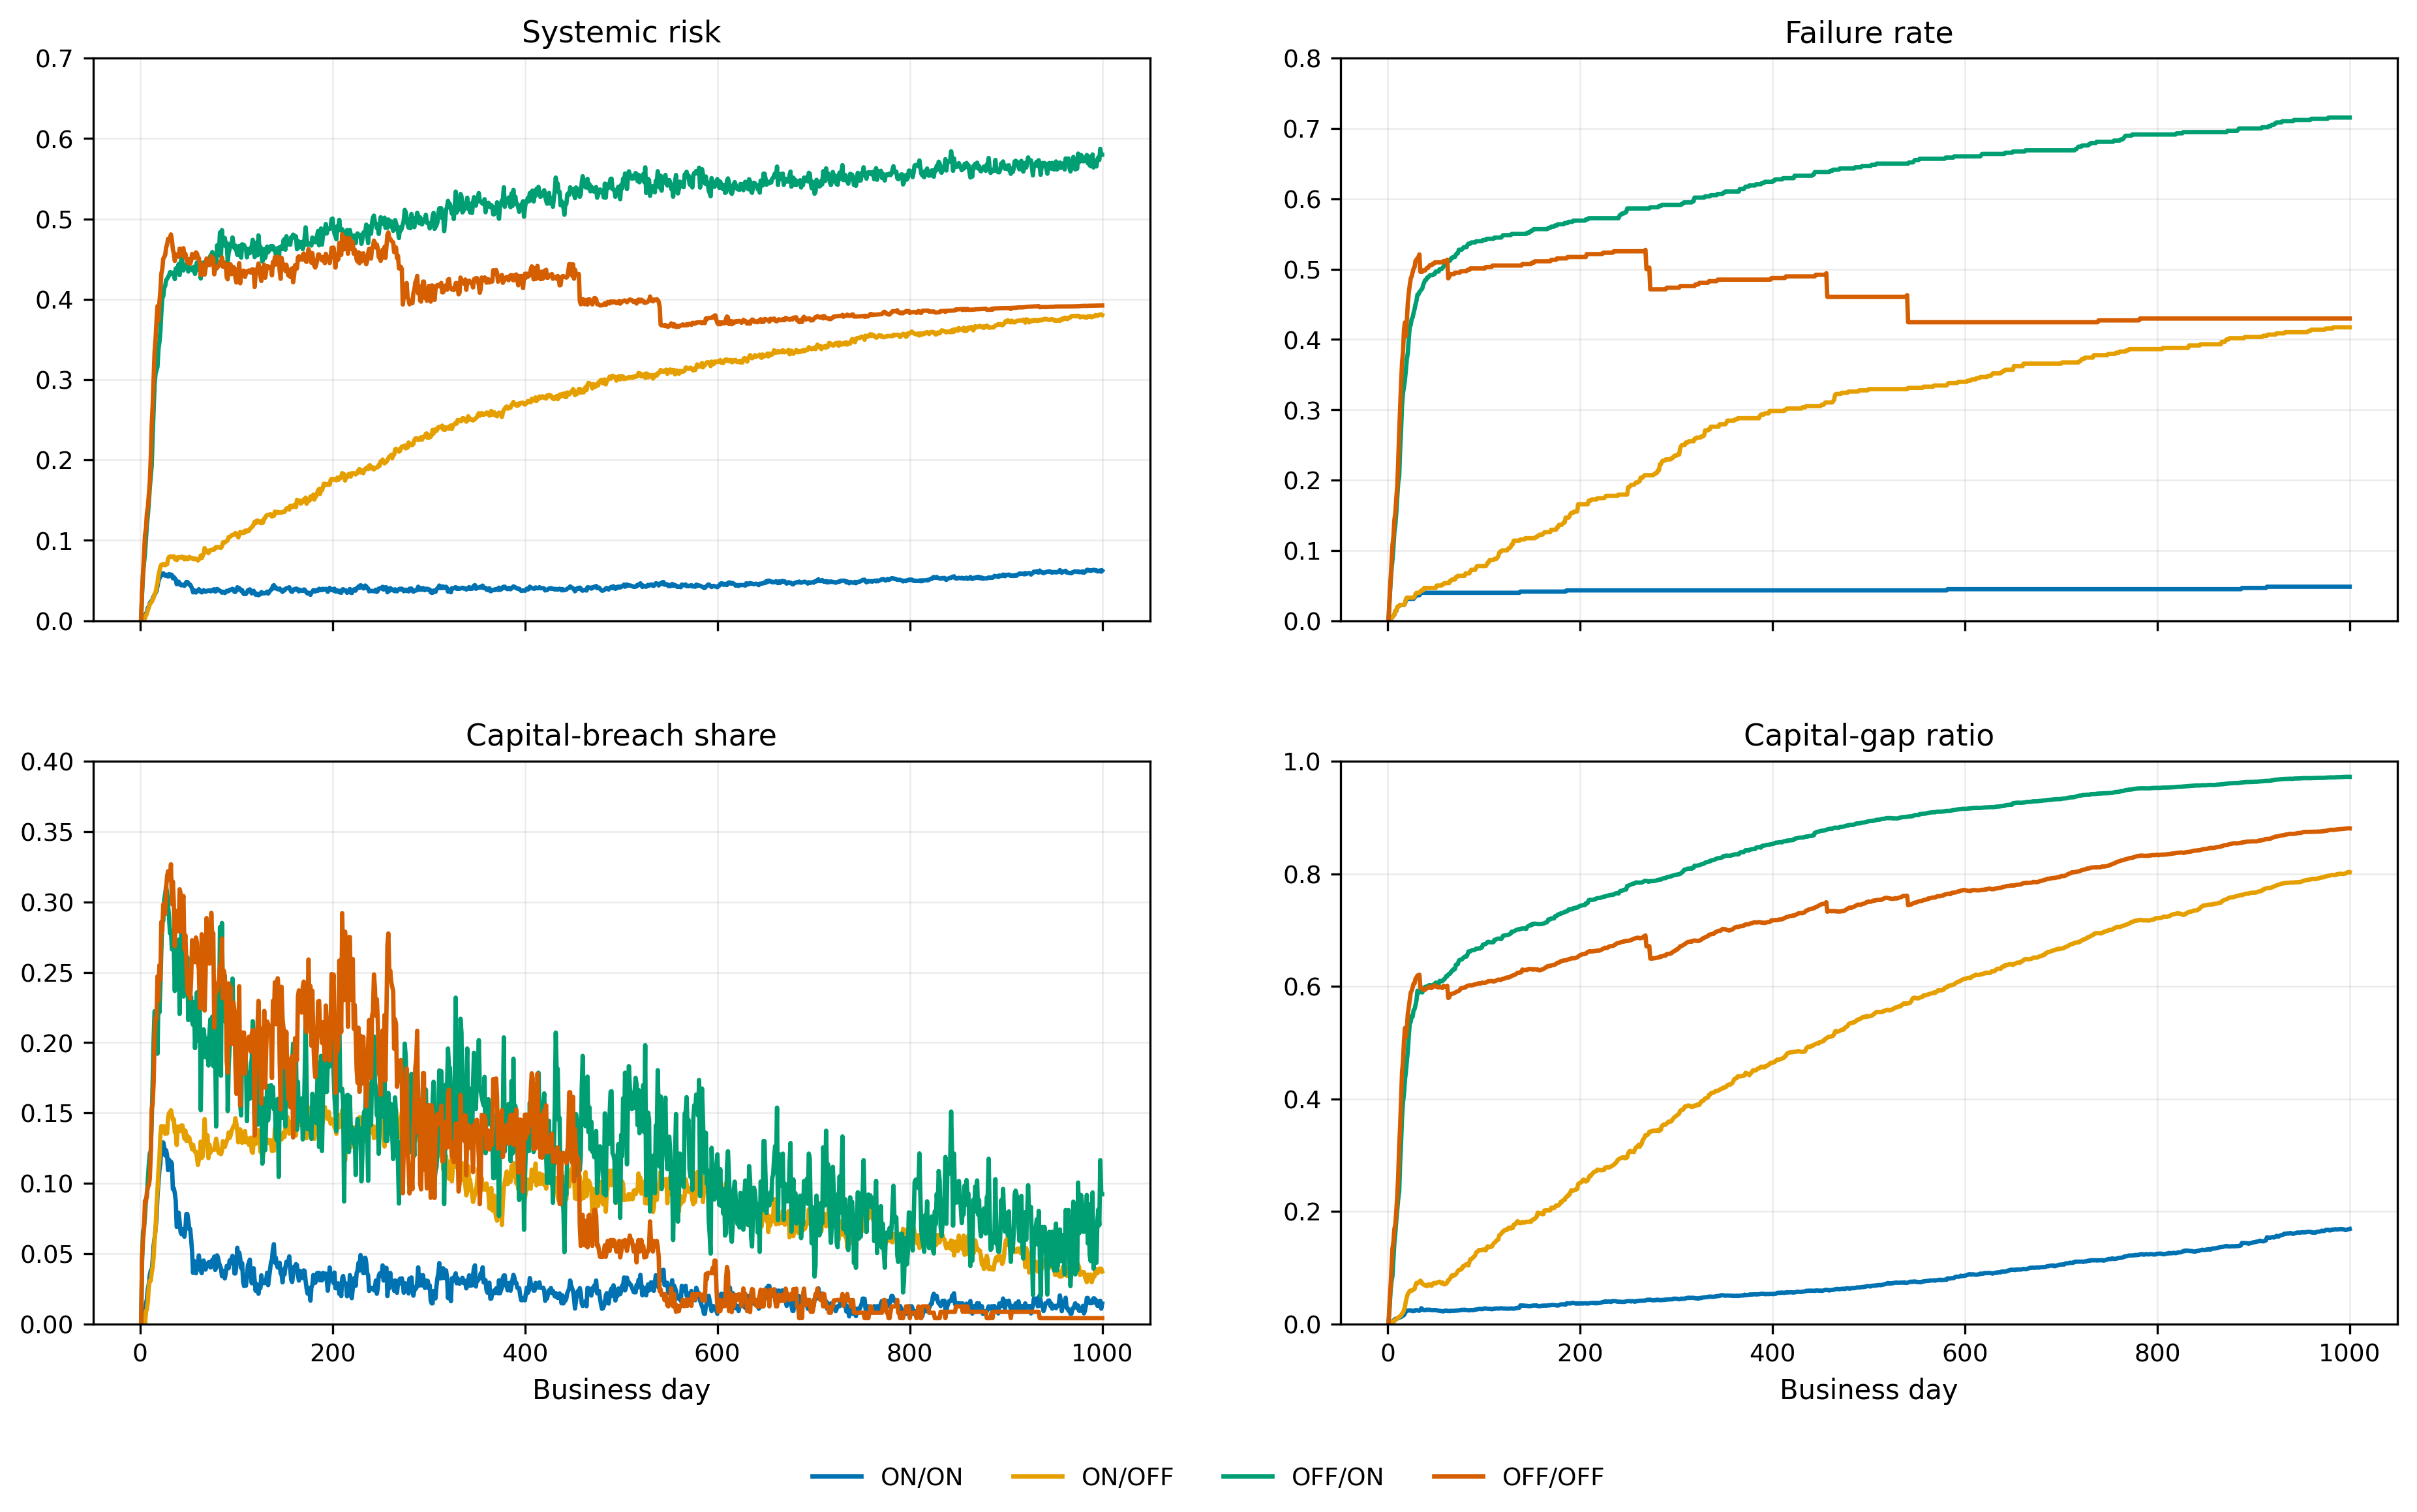
\includegraphics[width=0.96\textwidth]{figures/compare_four_baselines_centralized.png}
\caption{Four rollover/support configurations under centralized matching.}
\label{fig:four-cen}
\end{figure}

Across all four configurations, the RFQ mean-risk point estimate is below
the centralized estimate. The ON/ON paired mean difference is
\(-0.0051\), with interval \([-0.0128,0.0025]\). In the other three
configurations the differences are larger and their intervals exclude
zero: \(-0.0786\) \([-0.1058,-0.0514]\) for ON/OFF,
\(-0.1053\) \([-0.1323,-0.0783]\) for OFF/ON, and
\(-0.0878\) \([-0.1234,-0.0522]\) for OFF/OFF. These comparisons show
that the mechanism ranking is stable in this design, while the absolute
risk level depends strongly on rollover and support.

No ON/ON or ON/OFF replication stops before day 1000, so restricted mean
survival time is 1000 in those cells and cannot distinguish the
scenarios. Bank-days provide a more sensitive within-horizon outcome.
Relative to OFF/OFF, ON/ON adds an estimated 13,353.9 non-central-bank
days under RFQ, with a paired interval of \([10085.1,16800.8]\), and
16,004.1 fixed-horizon bank-days under centralized matching, with interval
\([12217.6,19890.1]\). Relative to rollover ON/support OFF, ON/ON adds
4,467.0 bank-days under RFQ and 6,930.4 under centralized matching. The
combined policy configuration therefore
preserves more operating-bank time within the observed horizon. Collapse
time remains unidentified in ON/ON and ON/OFF, while OFF/OFF centralized
matching records seven early stops (Table~\ref{tab:run-length}).

Table~\ref{tab:policy-event} summarizes the exported mean daily policy
series over the pre-specified 100-business-day window and the full
horizon. Unique-recipient counts, issuance dates, repayment rates, and
remaining budgets are not stored in the Monte Carlo artifacts, so those
event-log fields cannot be estimated. The available series show that both
mechanisms use liquidity support on 99 of the first 100 days. Centralized
matching uses more solvency support early in the window (7.80 versus 2.35
per day), while full-horizon integrated totals remain close.

\begin{table}[htbp]
\centering
\caption{ON/ON policy-support series from exported mean daily paths}
\label{tab:policy-event}
\small
\begin{tabular}{@{}lrrrr@{}}
\toprule
\textbf{Measure} & \textbf{RFQ [1,100]} & \textbf{CEN [1,100]} & \textbf{RFQ [1,1000]} & \textbf{CEN [1,1000]}\\
\midrule
Mean daily liquidity & 361.5 & 350.8 & 108.9 & 107.3\\
Mean daily solvency & 2.35 & 7.80 & 2.09 & 2.01\\
Mean daily total & 363.9 & 358.5 & 111.0 & 109.3\\
Positive-support days & 99 & 99 & -- & --\\
First positive day & 2 & 2 & 2 & 2\\
\bottomrule
\end{tabular}
\begin{minipage}{0.96\textwidth}
\footnotesize
\textit{Note:} Entries are cross-seed mean daily series stored in the
artifacts, not bank-level event logs. Support-off scenarios record zeros
on every day and are omitted. Unique-bank and repayment fields are
unavailable in the exported batch.
\end{minipage}
\end{table}

\section{Measurement Sensitivity}

The CAR-threshold and failure-weight exercises are measurement sweeps:
they re-evaluate the same recorded bank-state paths and do not rerun the
economic system, because \(\theta\) and
\(w_1\) change the definition of measured SR rather than bank decisions in
the baseline simulation.

Figure~\ref{fig:theta-sweep} separates RFQ and centralized paths into two
panels with a common vertical scale and threshold color map. Each panel
contains all eight threshold values. The black curve marks the baseline
\(\theta=0.08\).

\begin{figure}[htbp]
\centering
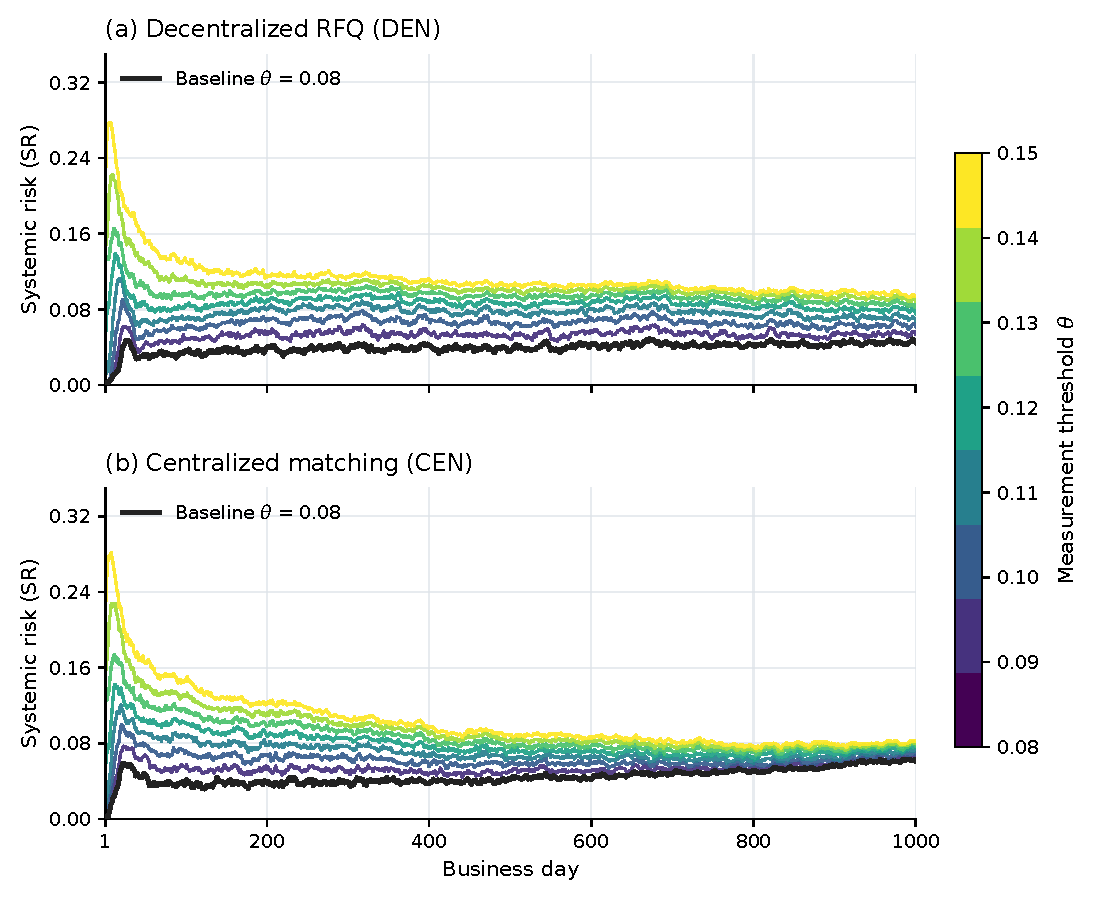
\includegraphics[width=\textwidth]{figures/compare_theta_sweep_sr_rollover_on_support_on.pdf}
\caption{CAR-threshold measurement sweep under ON/ON. RFQ and centralized matching are shown in separate panels using the same axes and threshold color scale.}
\label{fig:theta-sweep}
\end{figure}

At low and baseline thresholds, RFQ has lower average measured SR. For
example, at \(\theta=0.08\), the aggregate path means are 0.0396 and
0.0447 for RFQ and centralized matching. The difference narrows at
\(\theta=0.09\) and reverses at \(\theta=0.10\): at \(\theta=0.15\), the
corresponding means are 0.1139 and 0.1035. Thus the claim that RFQ is
safer is robust at the selected regulatory threshold but is not invariant
to broader classification of capital stress.

\begin{figure}[htbp]
\centering
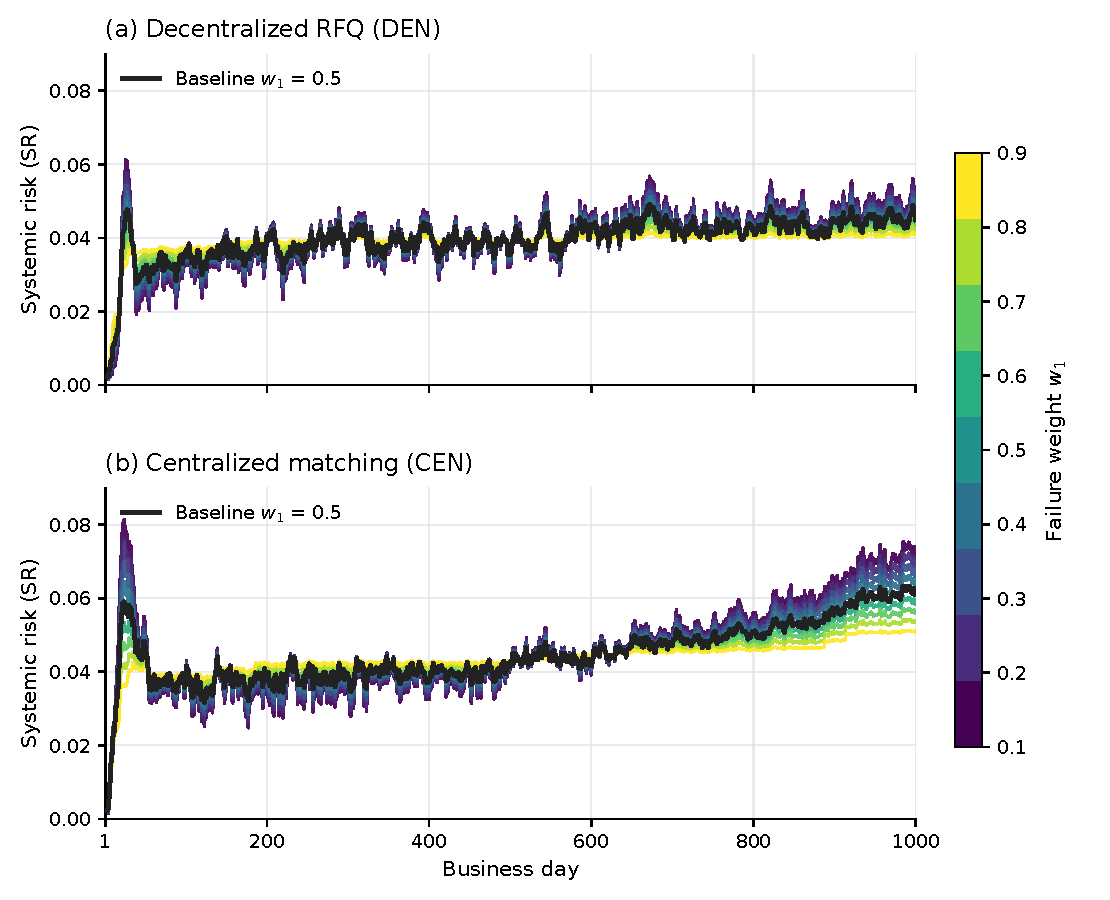
\includegraphics[width=\textwidth]{figures/compare_weight_sweep_sr_rollover_on_support_on.pdf}
\caption{Failure-weight measurement sweep under ON/ON, with separate
RFQ and centralized panels using identical axes and a common weight color
scale. All nine weights are shown; the black curve marks \(w_1=0.5\),
and \(w_2:w_3=3:2\) throughout.}
\label{fig:weight-sweep}
\end{figure}

Across \(w_1\in\{0.1,\ldots,0.9\}\), while preserving
\(w_2:w_3=3:2\), the average RFQ path remains below the centralized path.
The difference becomes smaller as more weight is placed on realized
failure and less on capital stress, consistent with the baseline result
that the clearest separation occurs in the capital-gap component.

\section{Structural Robustness to the Single-Loan Cap}

Unlike the preceding measurement sweeps, changing the single-loan cap
reruns the economic simulation because \(B\) changes feasible trade sizes
and network formation. The thesis uses this check only to examine whether
the composite-risk ranking is stable. The sweep uses an independent
20-seed batch shared across both mechanisms and all three cap values,
as documented in Section~6.1. Its \(B=1200\) cell has a paired day-1000
SR difference of \(-0.00544\); the formal baseline sample in
Table~\ref{tab:paired-baseline-risk} has a difference of \(-0.01727\).
These are estimates from different replications under the same parameter
setting. Table~\ref{tab:loan-cap-network}, in contrast, reports network and
funding statistics from the formal ON/ON baseline sample.

Figure~\ref{fig:loan-cap} shows 20 paired runs at each value of
\(B\in\{600,1200,1800\}\). The paired final-risk estimates are negative at
all three caps (\(-0.0112\), \(-0.0054\), and \(-0.0076\)), so the
point-estimate ranking is unchanged. The interval excludes zero only at
\(B=600\); the intervals at \(B=1200\) and \(B=1800\) include zero. The
structural claim is therefore limited to directional ranking robustness
rather than uniform statistical separation.

\begin{figure}[htbp]
\centering
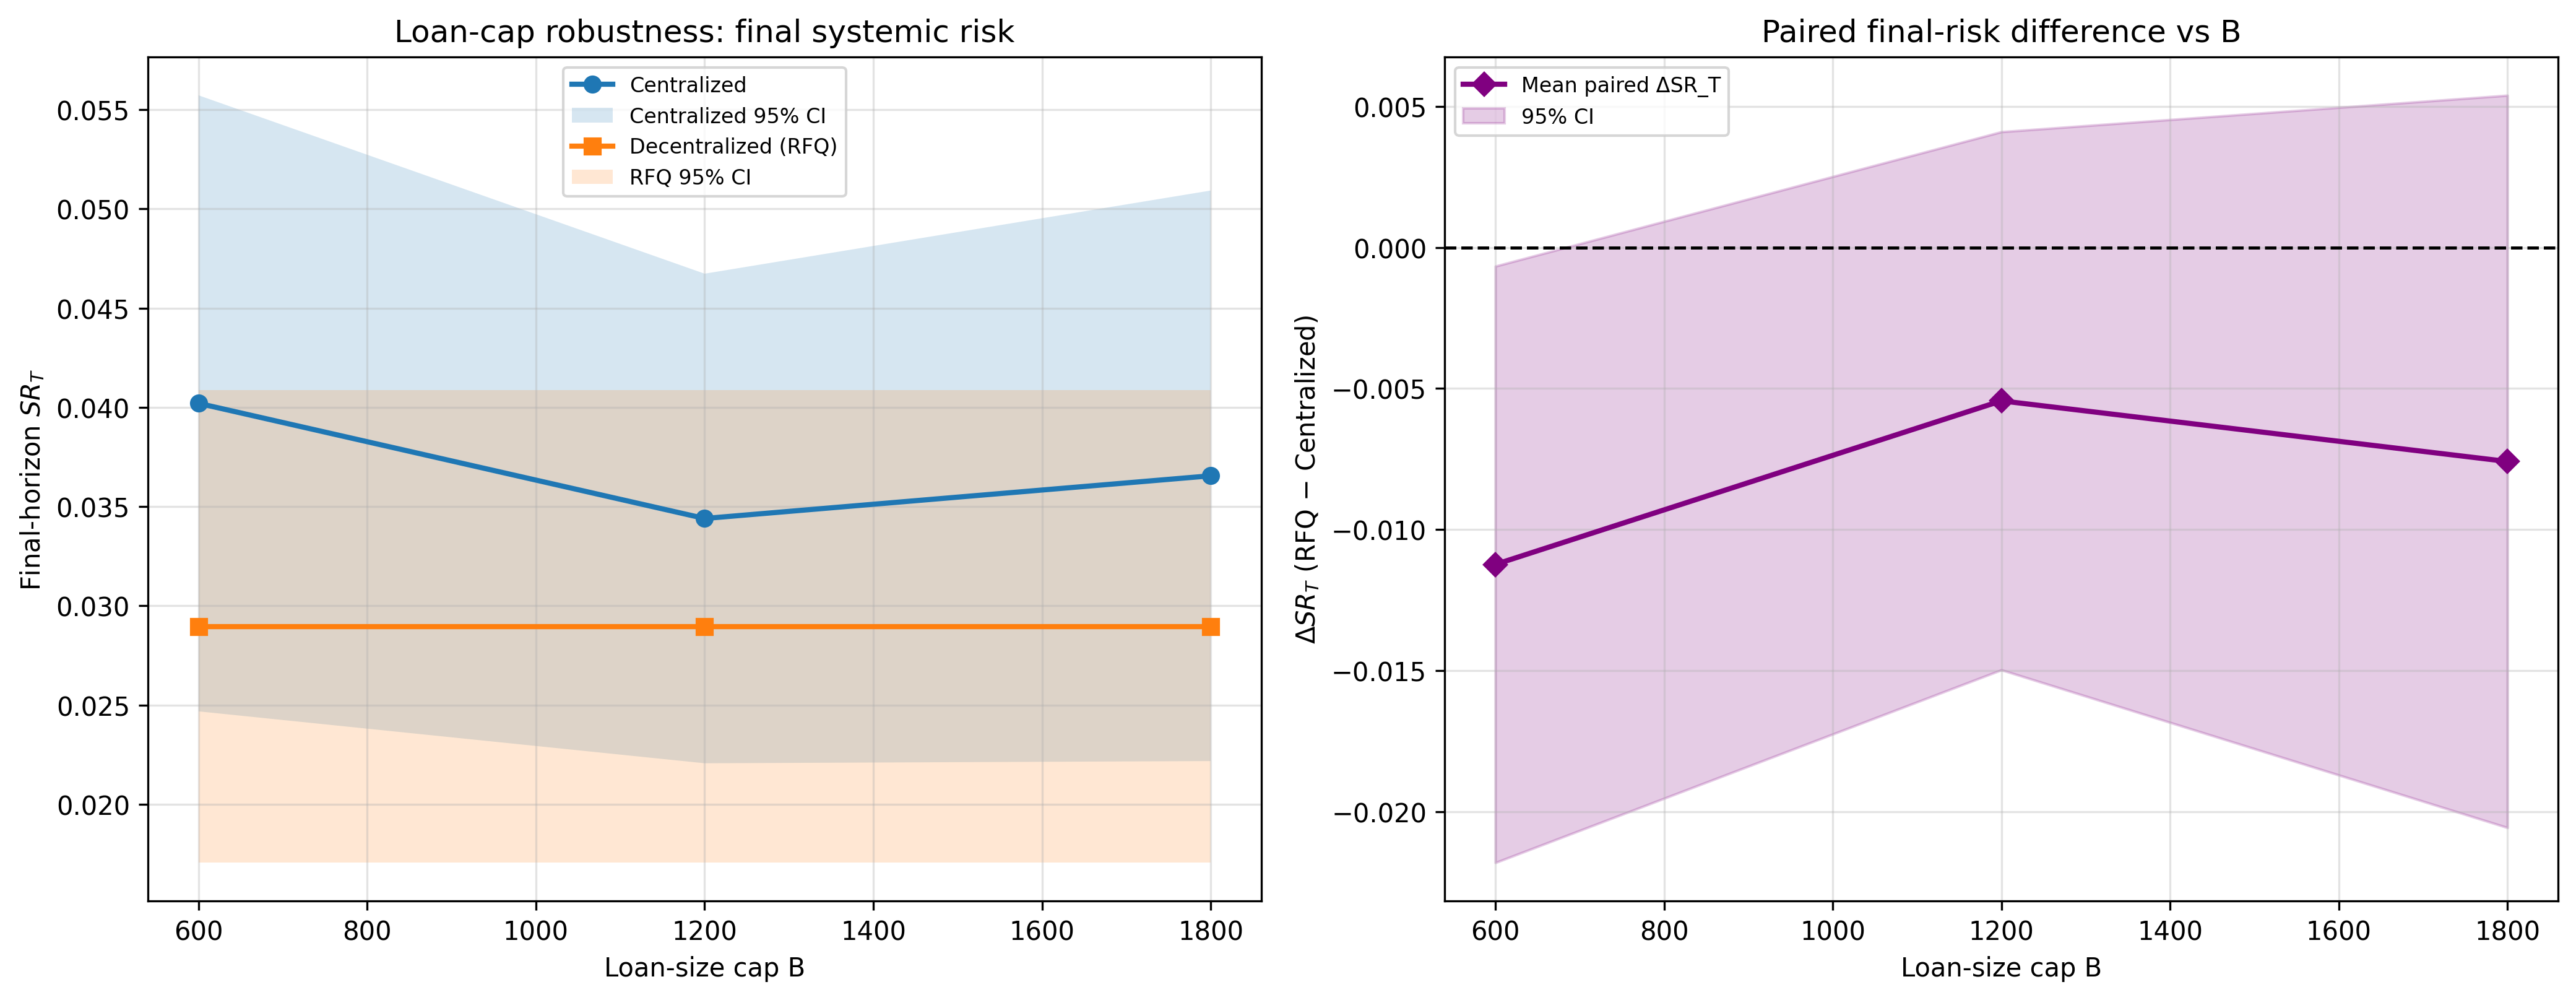
\includegraphics[width=\textwidth]{figures/loan_cap_robustness.png}
\caption{Loan-cap robustness check using a separate 20-seed batch shared
across all three caps and both mechanisms. The right panel shows paired
day-1000 SR differences, RFQ minus Centralized. The \(B=1200\) cell is
independent of the formal baseline sample in Table~\ref{tab:paired-baseline-risk}.}
\label{fig:loan-cap}
\end{figure}

\begin{table}[htbp]
\centering
\caption{Network and funding summary at the baseline loan cap \(B=1200\) (\(N=20\))}
\label{tab:loan-cap-network}
\small
\begin{tabular}{@{}lrrr@{}}
\toprule
\textbf{Measure} & \textbf{RFQ} & \textbf{Centralized} & \textbf{RFQ--Centralized (95\% CI)}\\
\midrule
Active directed links & 58.95 & 37.77 & $21.19$ $[14.13,\ 28.24]$\\
Network density & 0.0726 & 0.0465 & $0.0261$ $[0.0174,\ 0.0348]$\\
Exposure HHI & 0.050 & 0.094 & $-0.0435$ $[-0.0572,\ -0.0298]$\\
Largest bilateral exposure & 115.89 & 1,118.80 & $-1{,}002.91$ $[-1{,}167.96,\ -837.87]$\\
Funding satisfaction & 0.530 & 0.597 & $-0.067$ $[-0.111,\ -0.024]$\\
Cumulative volume & 325,406 & 314,721 & $10{,}685$ $[-41{,}740,\ 63{,}110]$\\
\bottomrule
\end{tabular}
\begin{minipage}{0.96\textwidth}
\footnotesize
\textit{Note:} This \(B=1200\) cell reuses the formal ON/ON sample in
Table~\ref{tab:network-results}. Intervals are paired normal-approximation
95\% intervals. These observations are distinct from the independent
loan-cap sweep batch in Figure~\ref{fig:loan-cap}.
\end{minipage}
\end{table}

\section{Discussion}

Three conclusions follow from the combined evidence. First, under the
baseline measurement, RFQ has lower estimated systemic risk and a lower
day-1000 capital-gap ratio, although the composite-risk confidence
interval is marginally inconclusive. Second, the mechanisms differ much
more clearly in structure: RFQ creates more, smaller, and less
concentrated bilateral exposures while accepting lower aggregate funding
coverage. Third, rollover and policy support preserve additional
bank-days within the 1000-day horizon. Collapse-time ranking is not
identified in ON/ON and ON/OFF because those paths are fully censored;
OFF/OFF centralized matching does record early stops
(Table~\ref{tab:run-length}).

The results therefore support a bounded conclusion rather than a universal
dominance claim. Decentralized screening and local execution can reduce
concentration and capital-gap risk near the baseline regulatory threshold,
but their measured advantage depends on the definition of capital stress
and comes with lower funding satisfaction. This trade-off is economically
more informative than choosing a mechanism from a single endpoint alone.
